\newpage
\subsection{Messungen}

\subsubsection{Modell}

%\begin{figure}[h!]
%	\centering
%	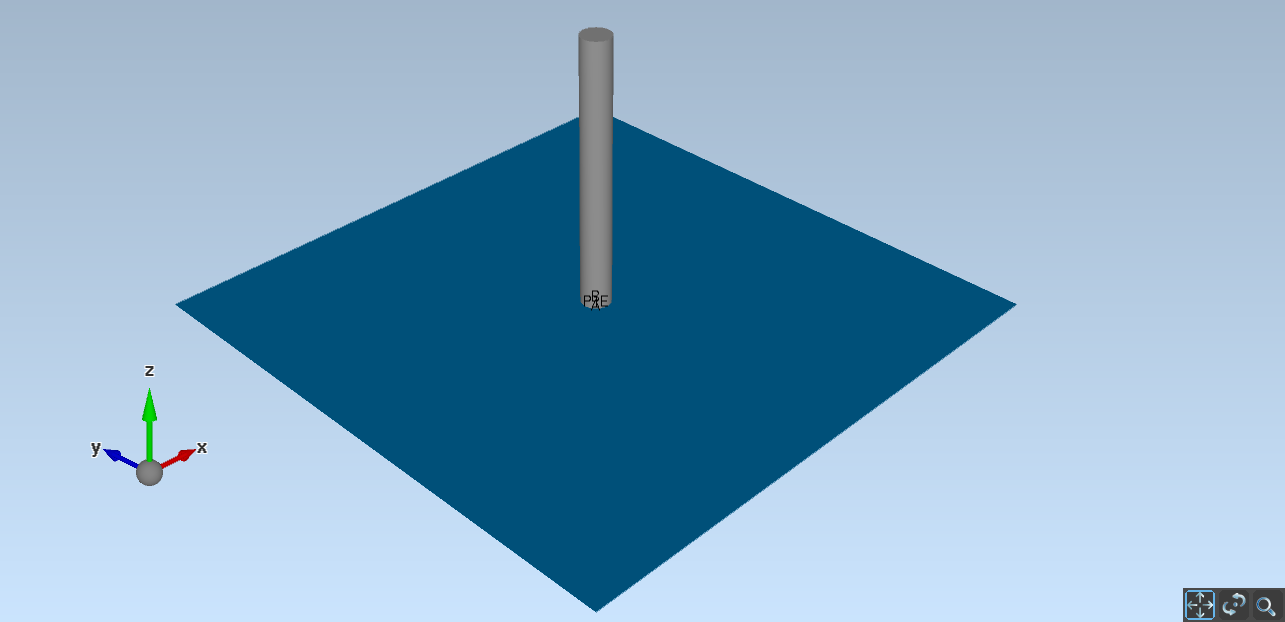
\includegraphics[width=0.5\textwidth]{../fig/plt/monopol_a_sim_3d_model.png}
%	\caption{}
%\end{figure}

\begin{figure}[h!]
	\centering
	\begin{subfigure}[b]{0.22\textwidth}
		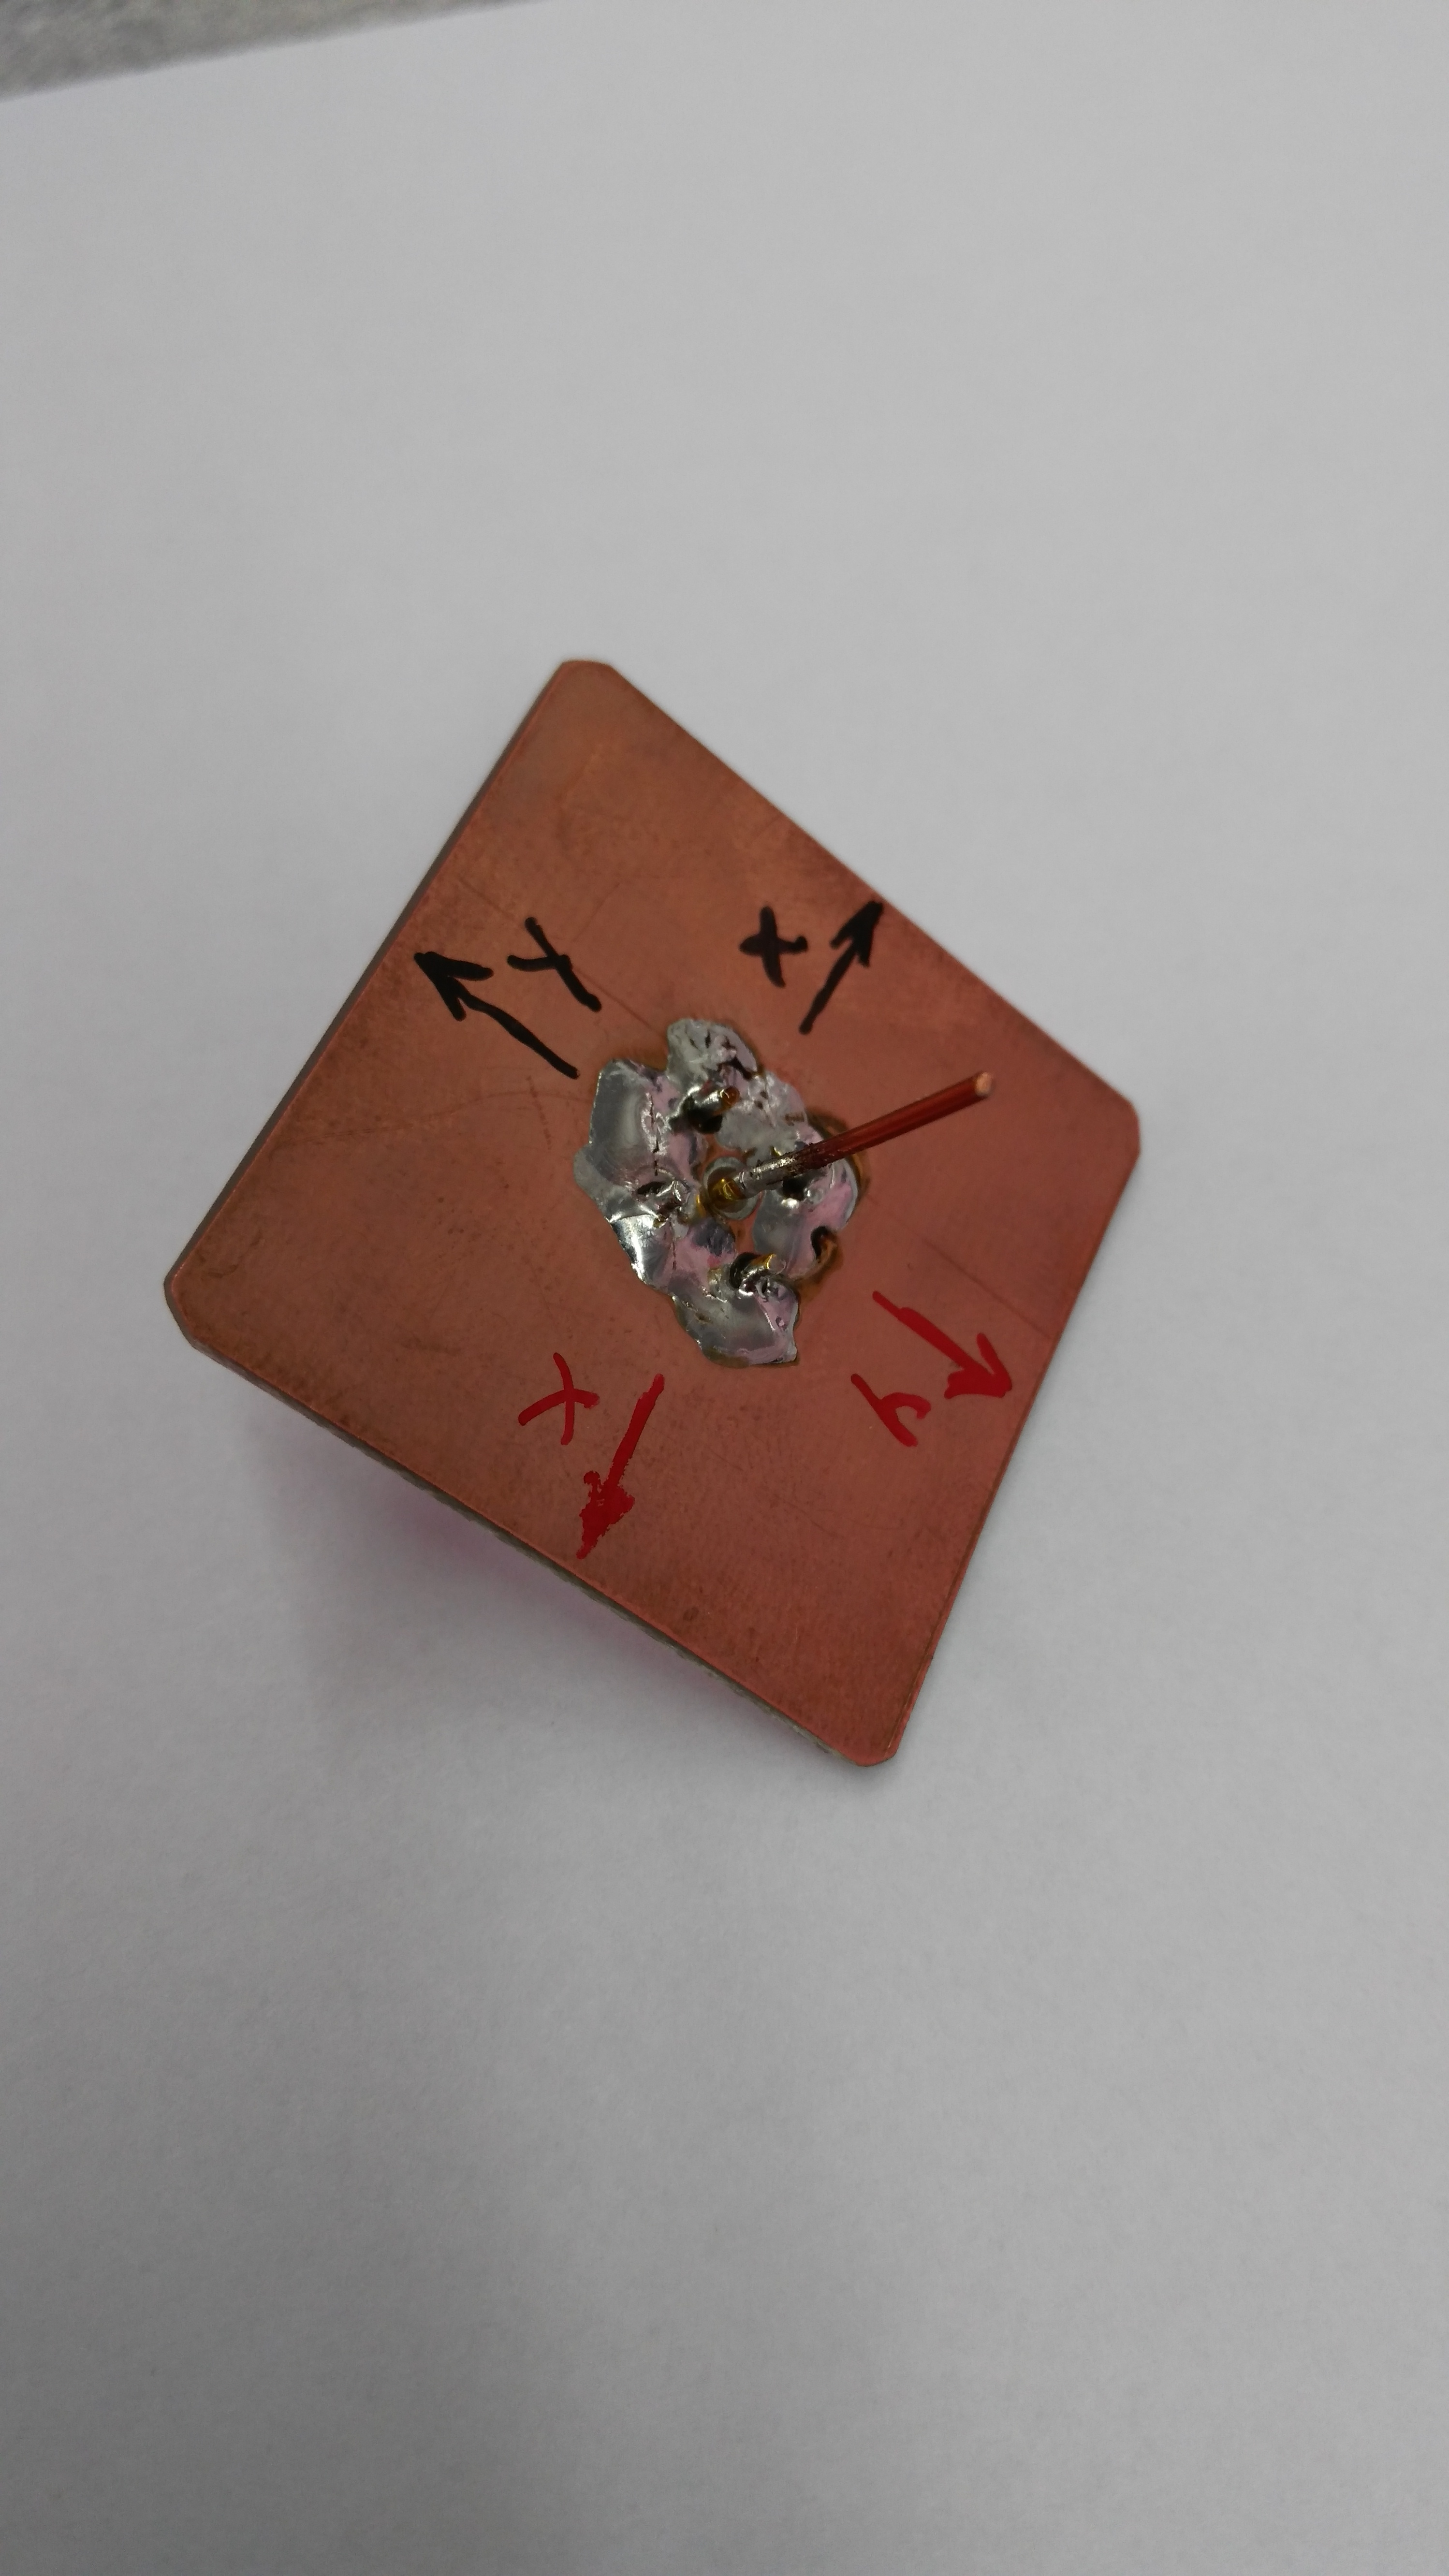
\includegraphics[width=1\textwidth]{../fig/pic/monopol_model_1.jpg}
		%\caption{a}
	\end{subfigure}
	\begin{subfigure}[b]{0.22\textwidth}
		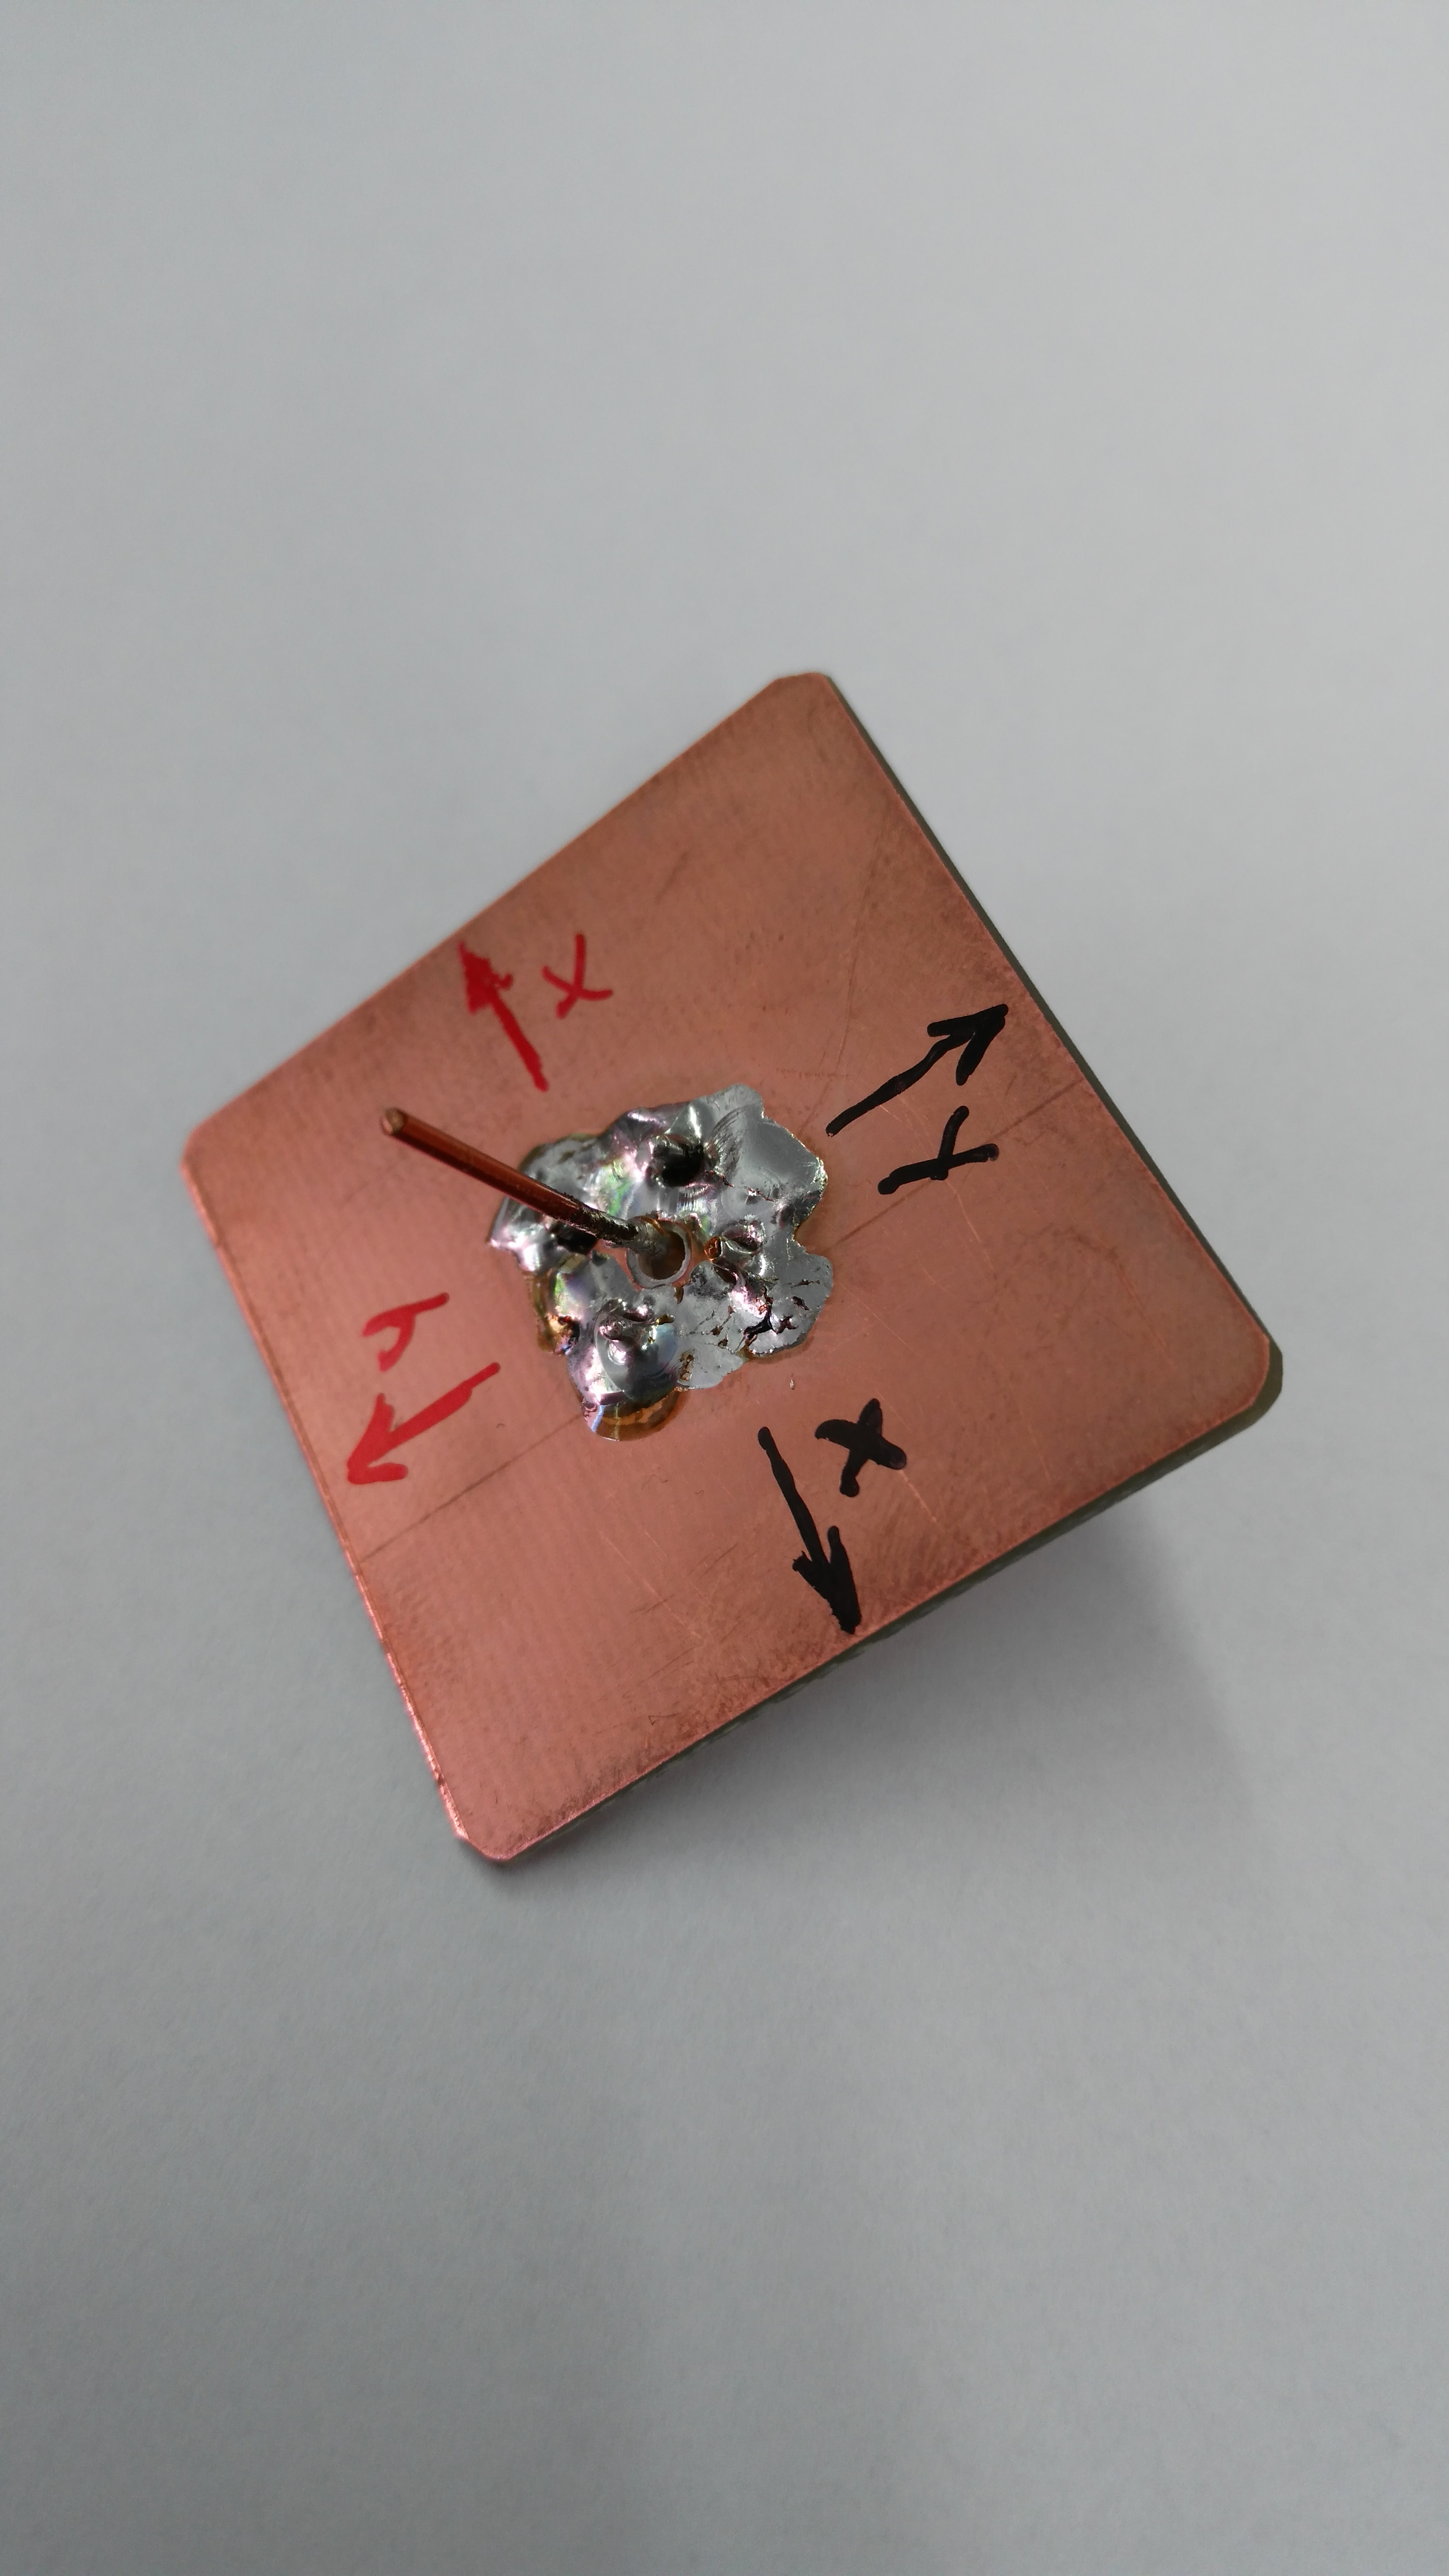
\includegraphics[width=1\textwidth]{../fig/pic/monopol_model_2.jpg}
		%\caption{b}
	\end{subfigure}
	\begin{subfigure}[b]{0.22\textwidth}
		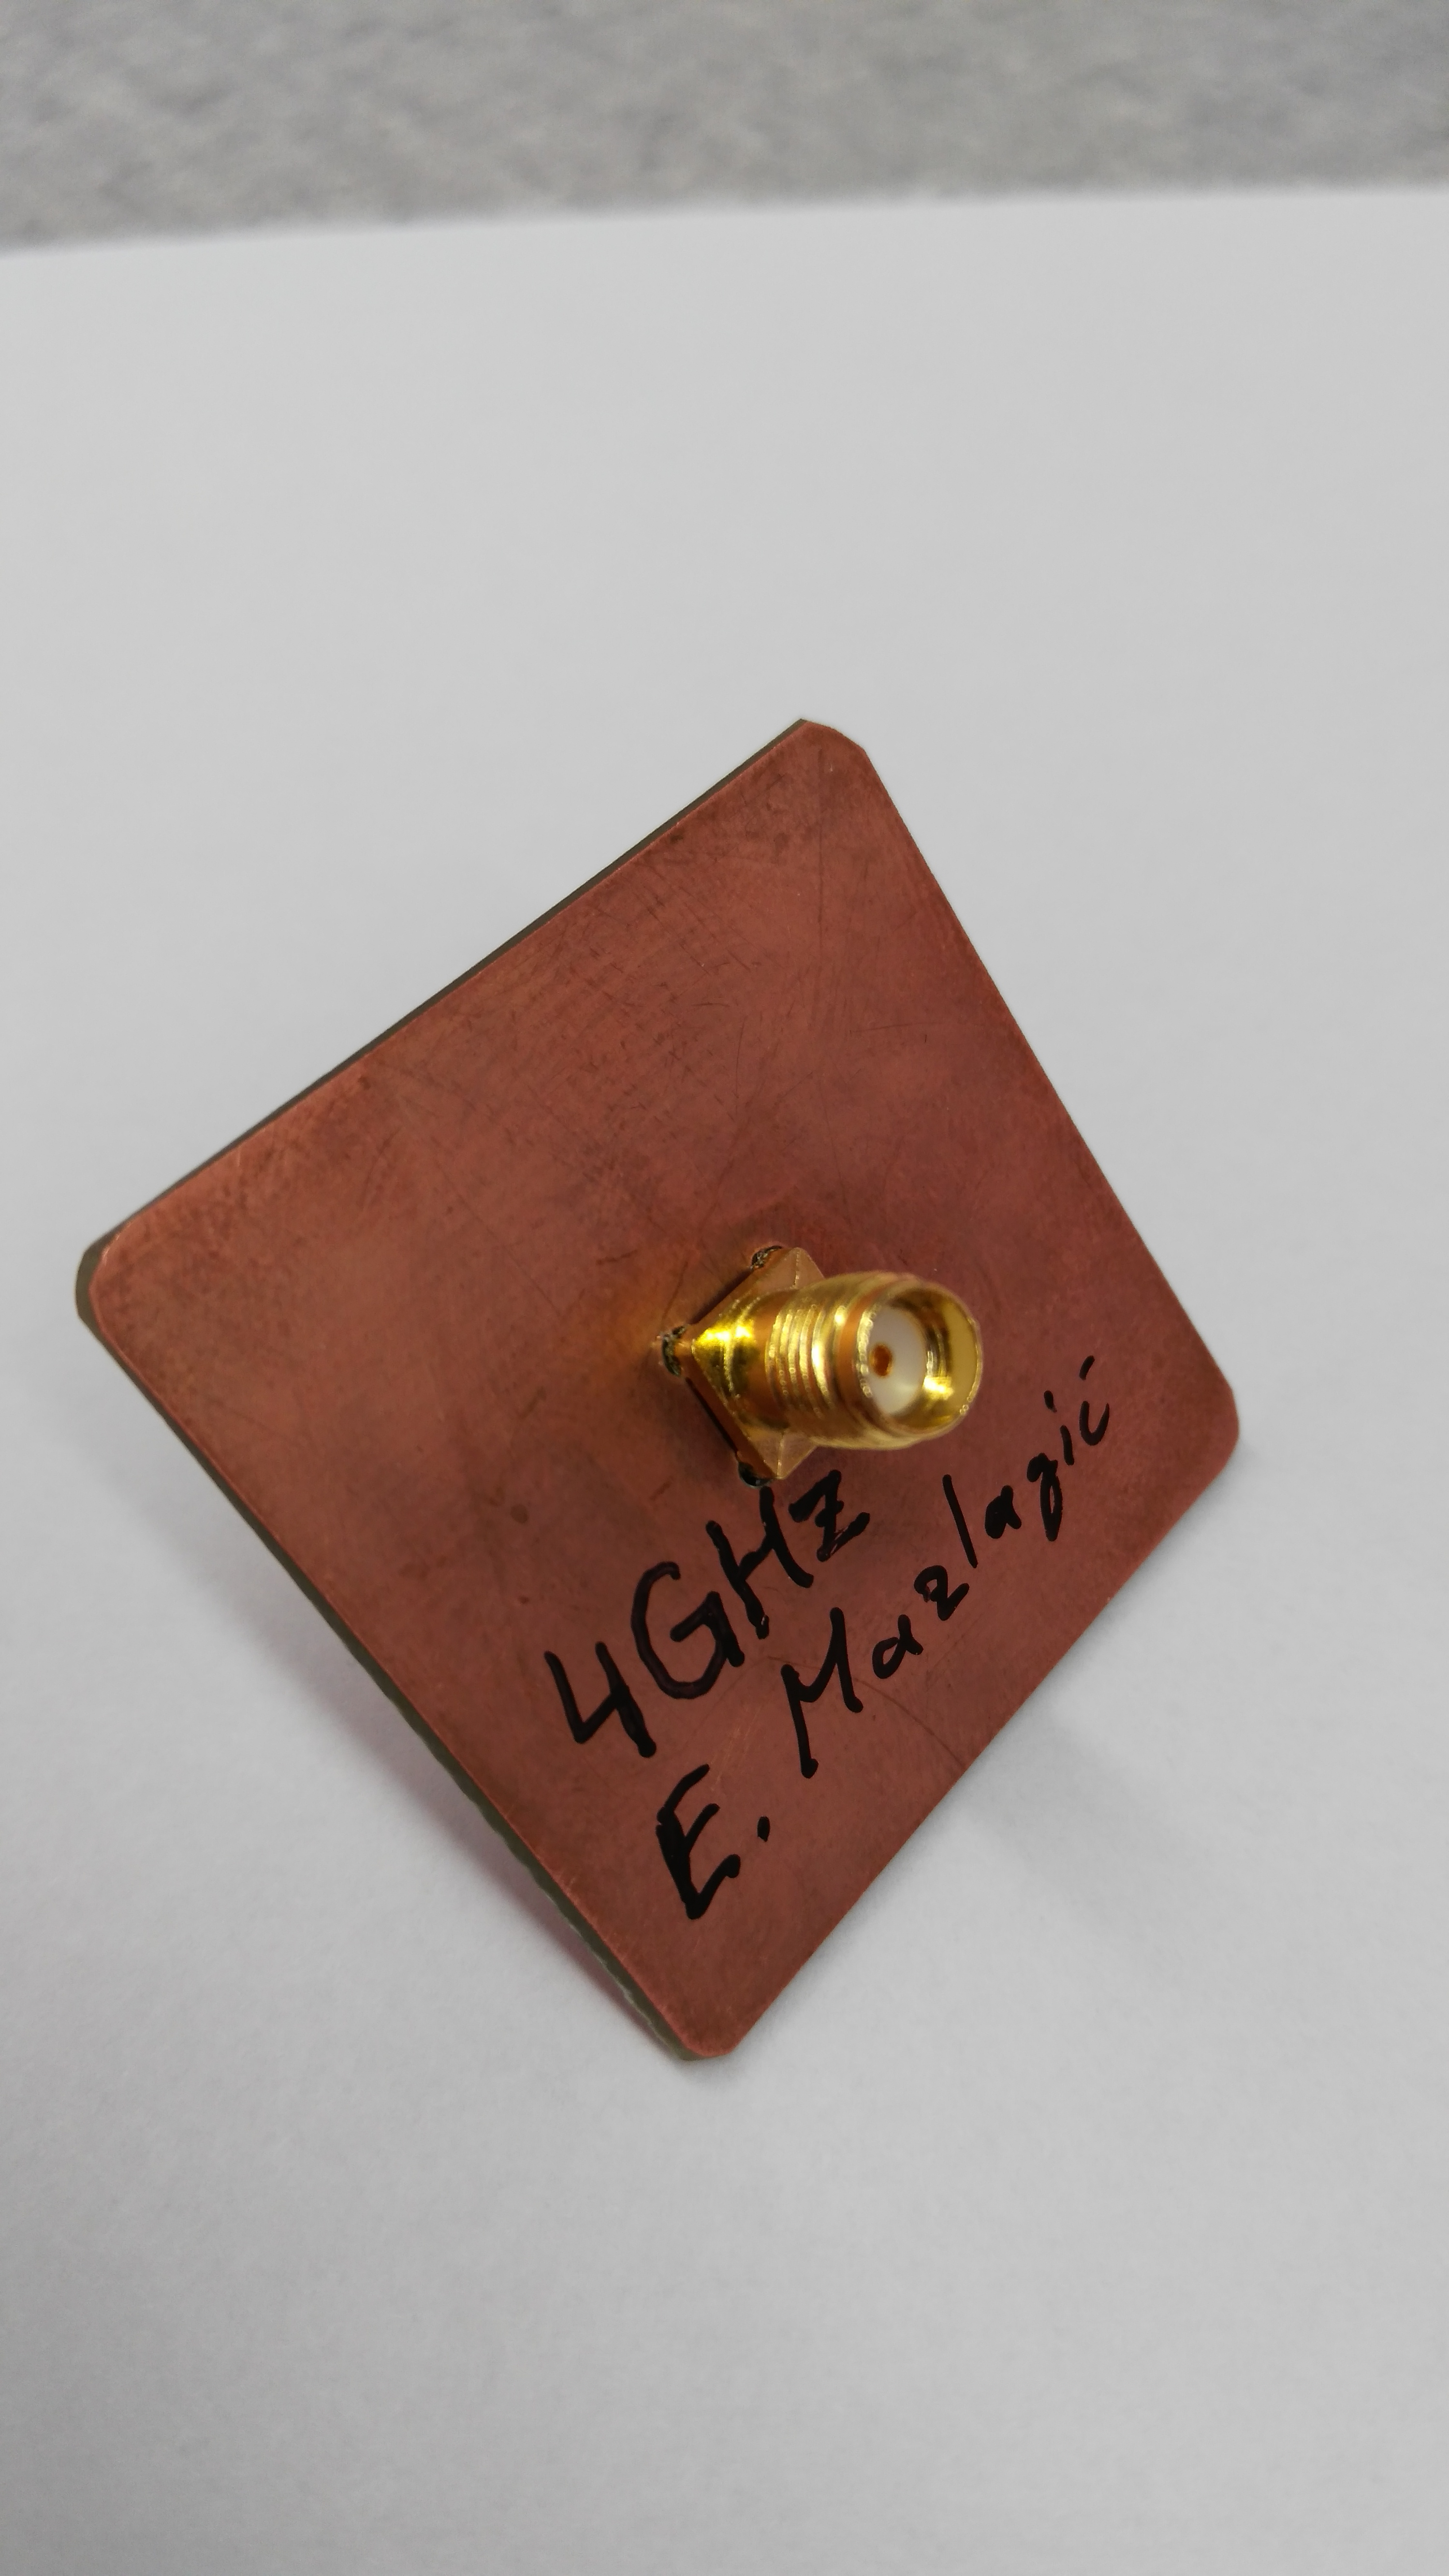
\includegraphics[width=1\textwidth]{../fig/pic/monopol_model_3.jpg}
		%\caption{c}
	\end{subfigure}
	\begin{subfigure}[b]{0.22\textwidth}
		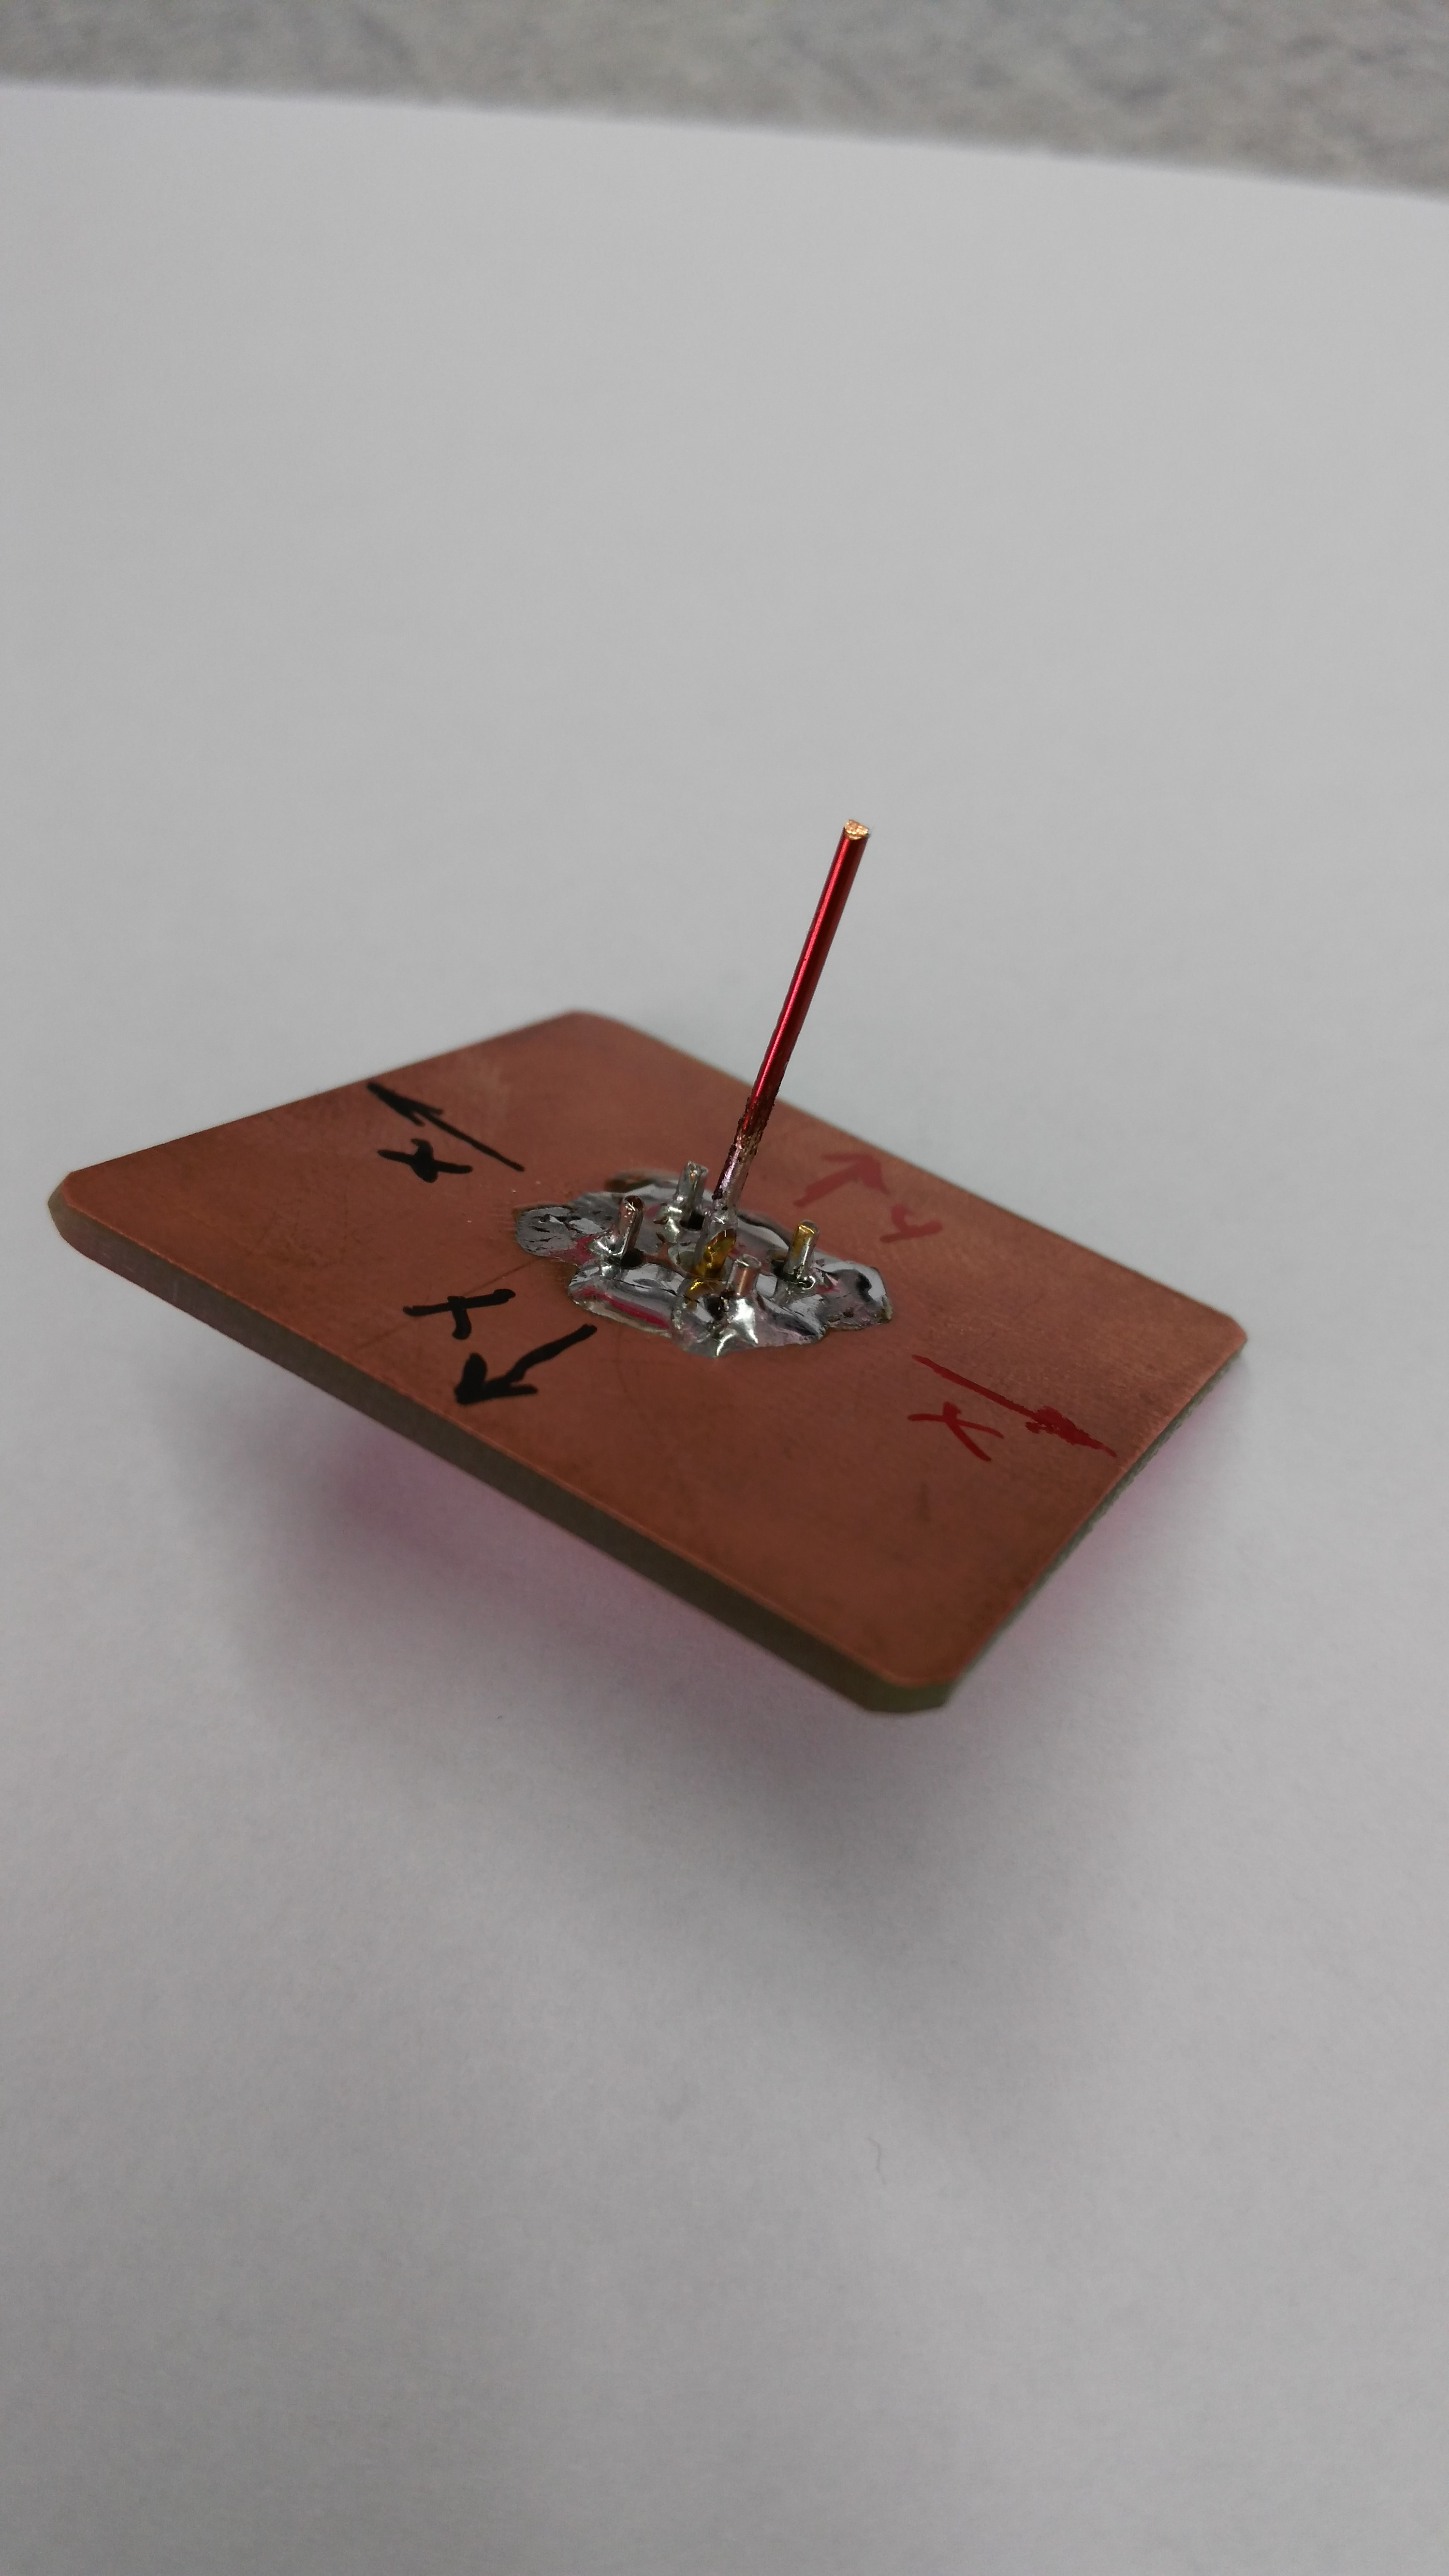
\includegraphics[width=1\textwidth]{../fig/pic/monopol_model_4.jpg}
		%\caption{d}
	\end{subfigure}
	\caption{Bilder der erstellten Monopolantenne.}
	\label{fig:monopol_model}
\end{figure}

Die Bilder der Abbildung \ref{fig:monopol_model} zeigen das erstellte Modell
der entworfenen Monopolantenne. Diese besteht aus einer beidsitig mit Kupfer
beschichteten Trägerplatte (Groundplane), einem lackiertem Wickeldraht
aus Kupfer (Stab) und einem SMA Stecker (Einspeisepunkt). Der Stab ist auf
die Ader des SMA Steckers gelötet. Die vier Beine des SMA Steckers, welche
als GND Anschluss dienen, sind mit dem Kupfer der Groundplane verlötet.

Die Stablänge wurde zunächst mit $2 \cdot l_S$ geweählt, damit diese auf die
richtige Länge hin gekürzt werden kann, um die gewünschte Resonanzfrequenz
zu erzielen (die Abbildung \ref{fig:monopol_model} zeigt den bereits gekürzten
Stab). Zudem wurde das Modell mit zwei Koordinatensystemen ausgestattet
($xzy$ in rot sowie $xyz$ in schwarz). Hierbei entspricht die Richtung des
Stabes der $z$-Achse der beiden Koordinatensysteme. 
Die gekennzeichneten Koordinatensysteme dienen der Orientierung bei der
Messung im StarLab. Der Grund für zwei vorbereitete Systeme liegt darin,
dass je nach Kabelführung der Messeinrichtung keine beliebige Ausrichtung
vorgenommen werden kann. Damit das Messsystem (insbesondere das Kabel für
die Einspeisung und Messung) keinen unnötigen Krafteinwirkungen ausgesetzt
wird, können so zwei respektive vier Ausrichtungen des Messobjekts verwendet
werden, womit eine maximale Drehung von
$\frac{\SI{360}{\degree}}{(4 \cdot 2)} = \SI{45}{\degree}$ möglich ist.

%\begin{figure}[h!]
%	\centering
%		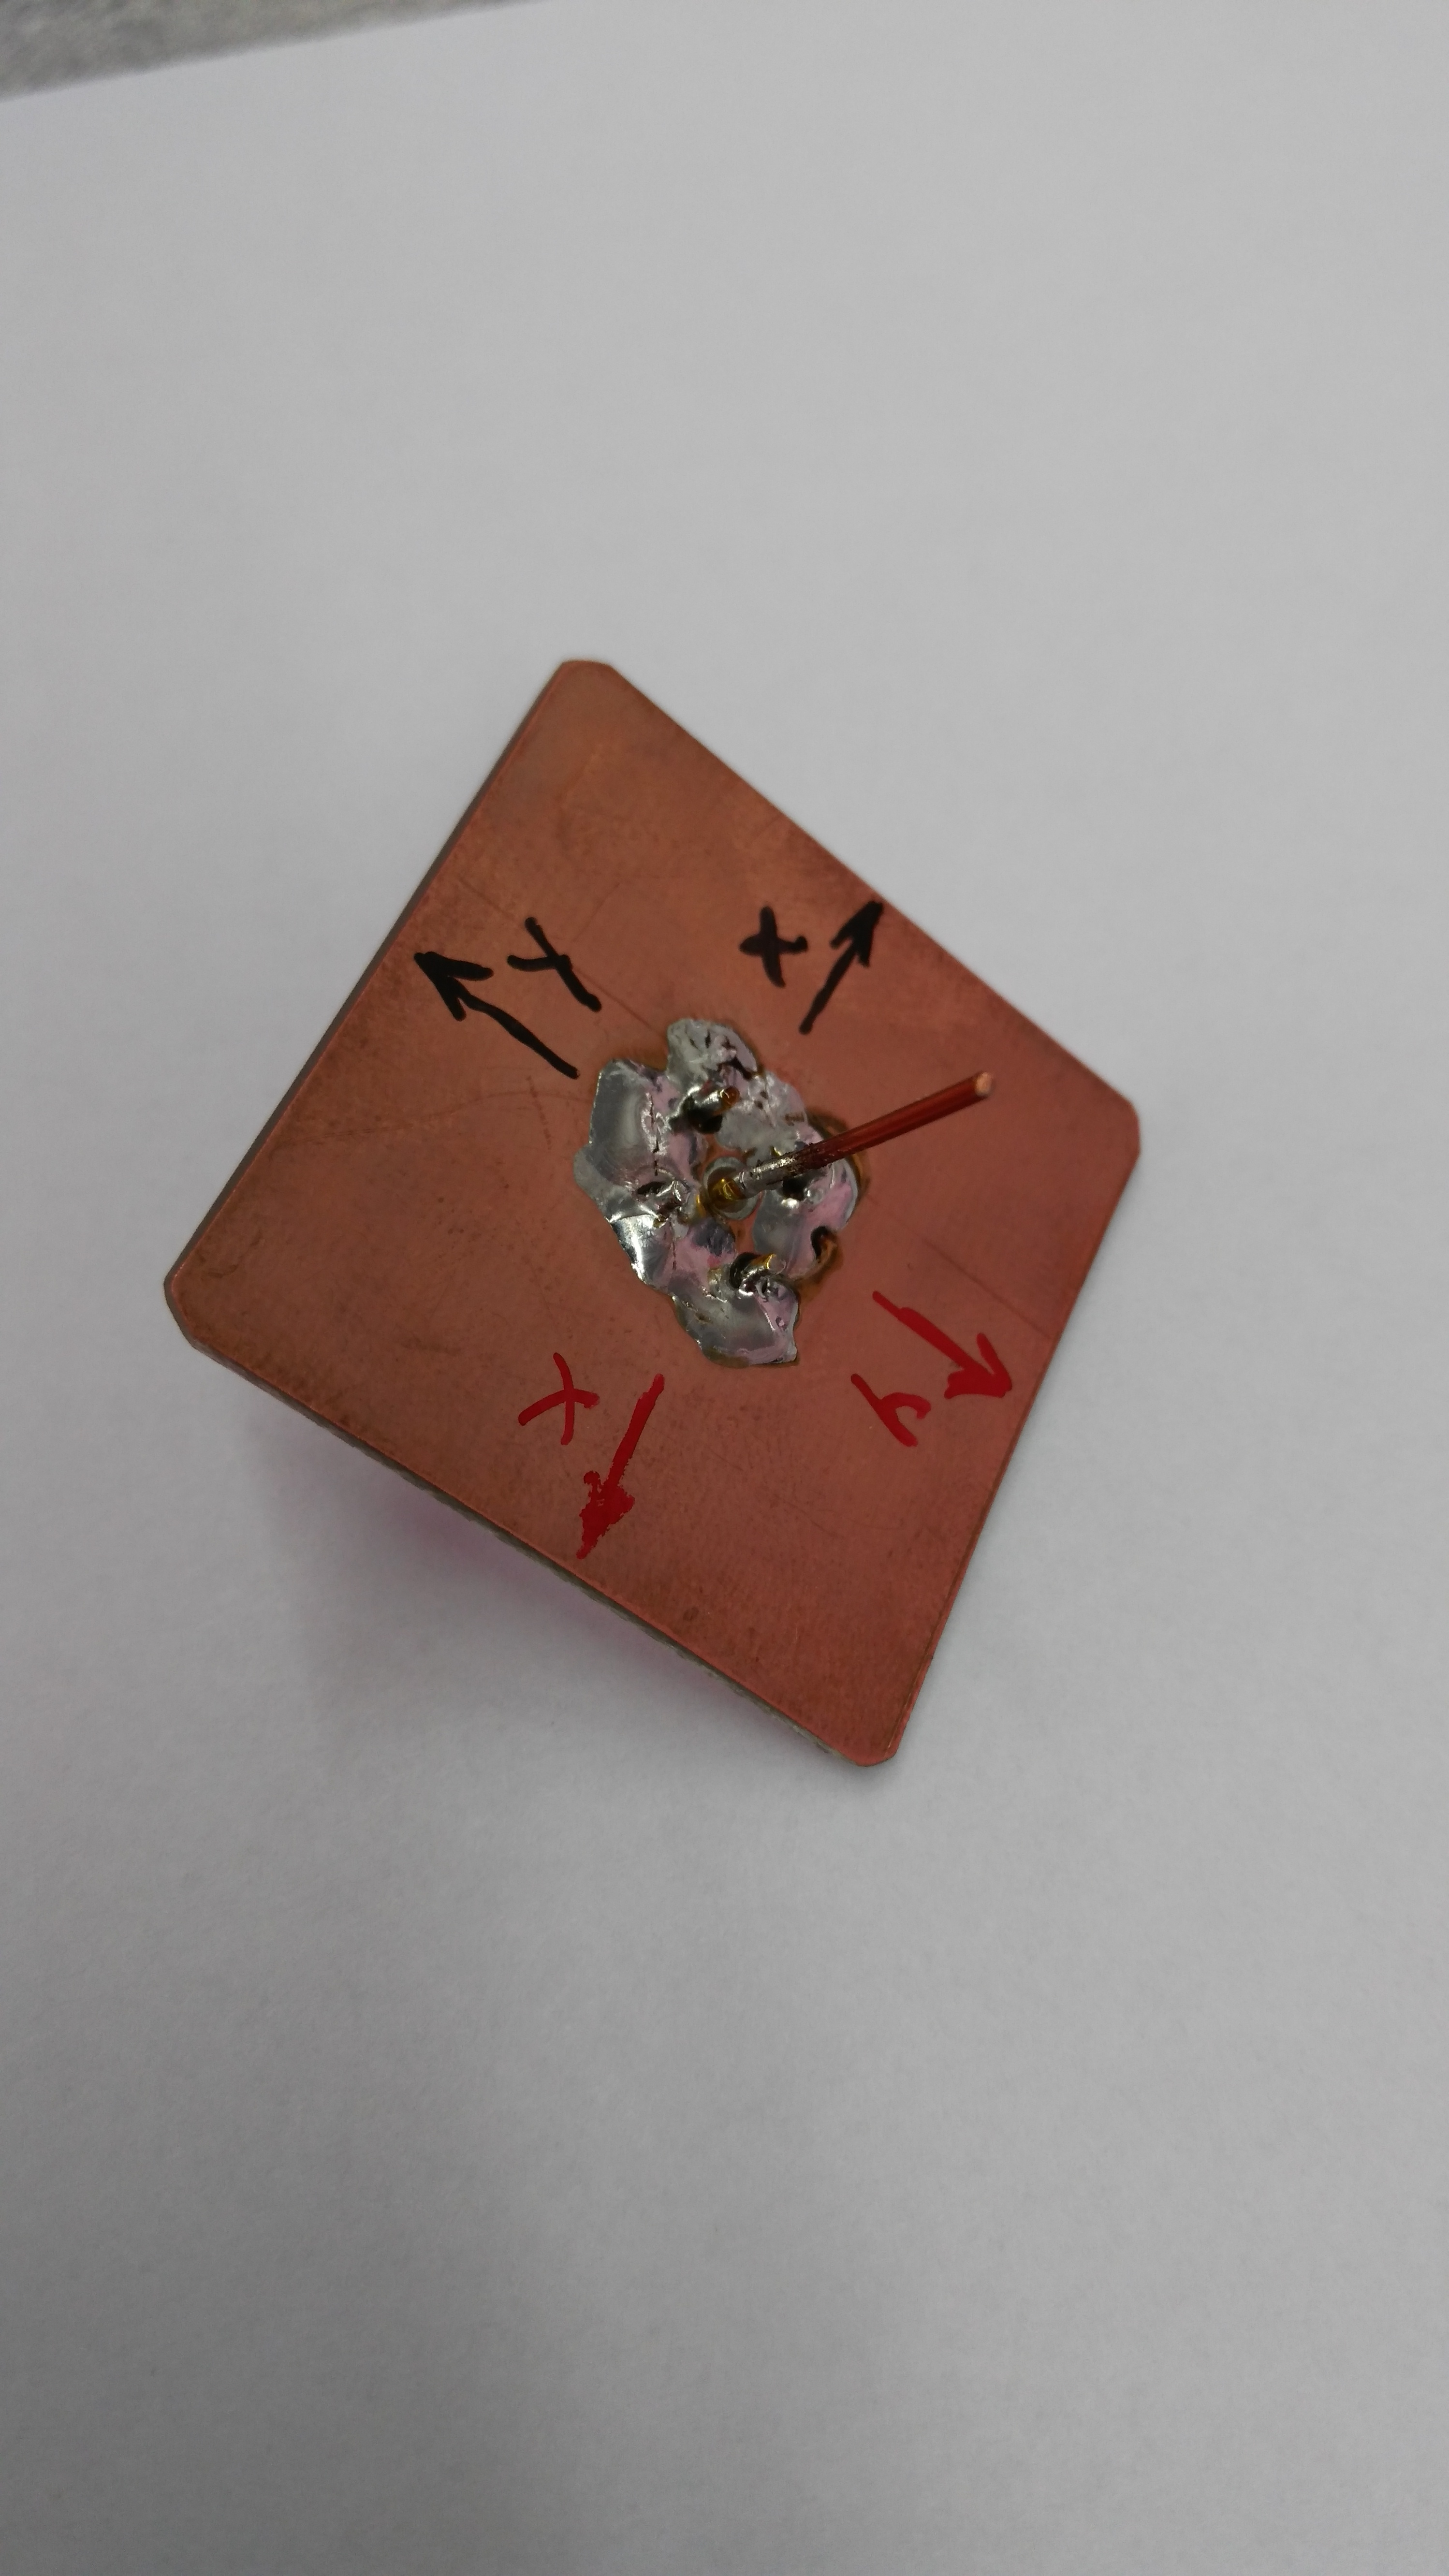
\includegraphics[width=0.22\textwidth]{../fig/pic/monopol_model_1.jpg}
%		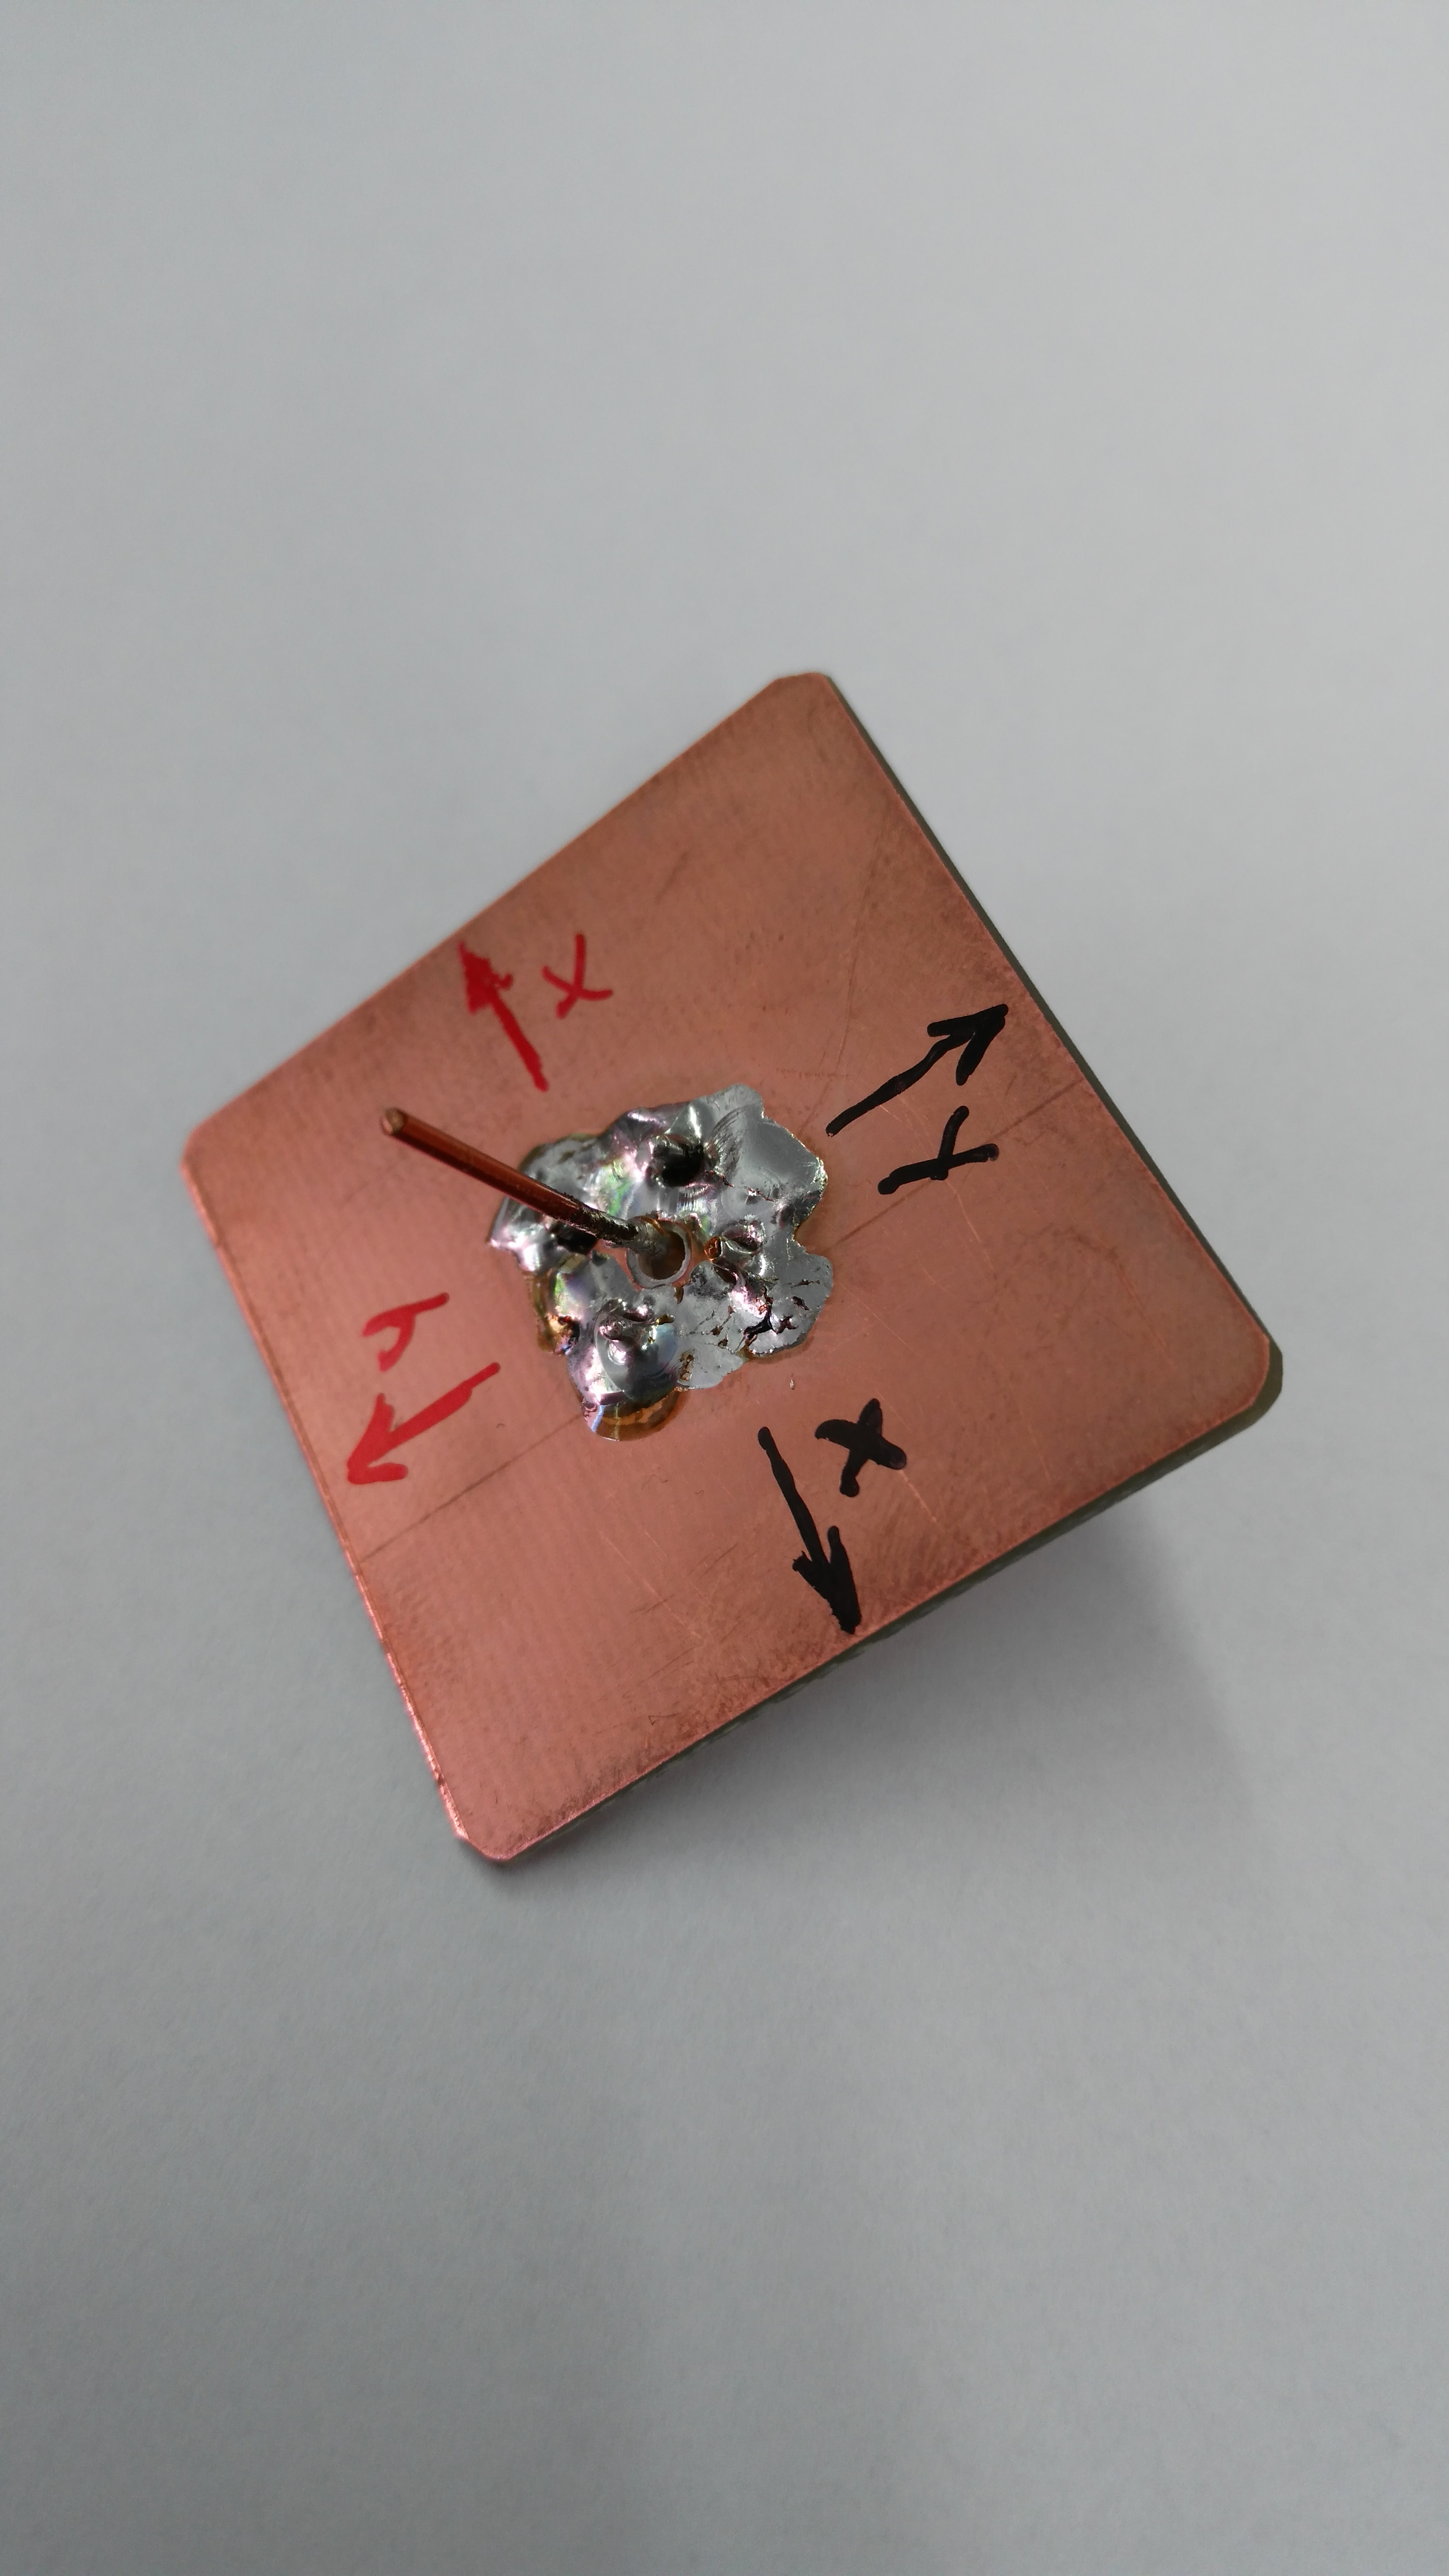
\includegraphics[width=0.22\textwidth]{../fig/pic/monopol_model_2.jpg}
%		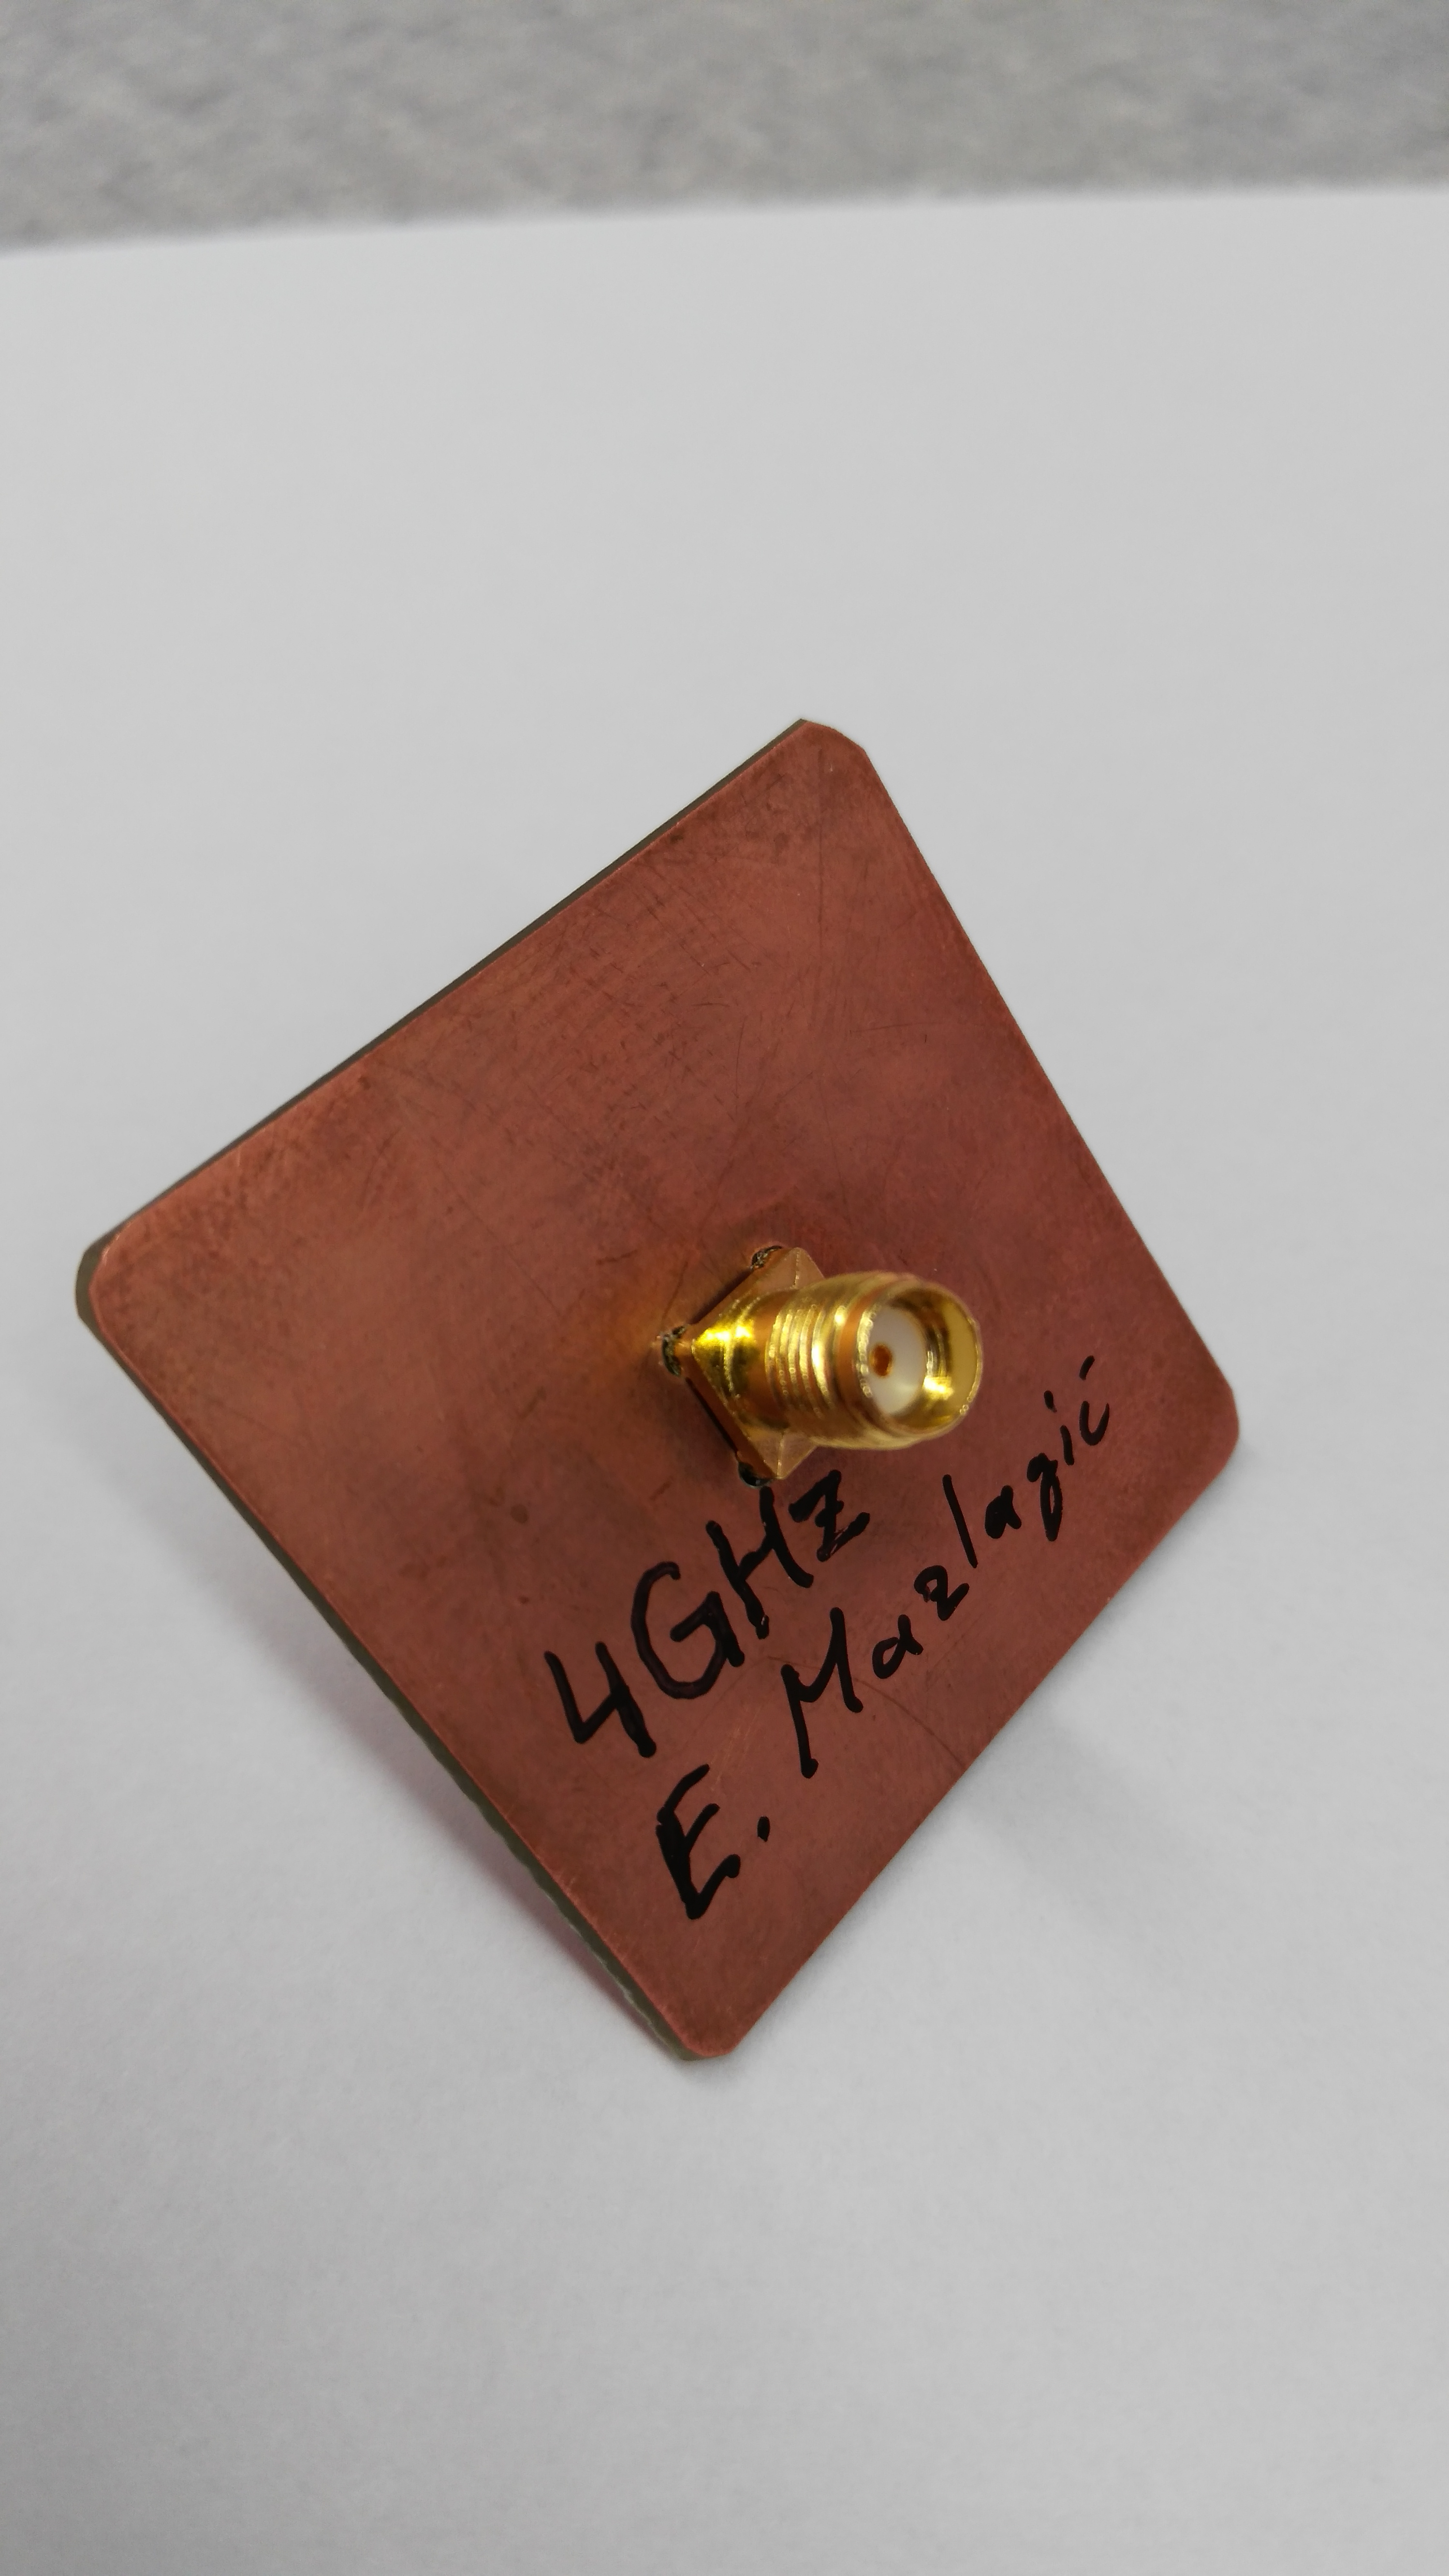
\includegraphics[width=0.22\textwidth]{../fig/pic/monopol_model_3.jpg}
%		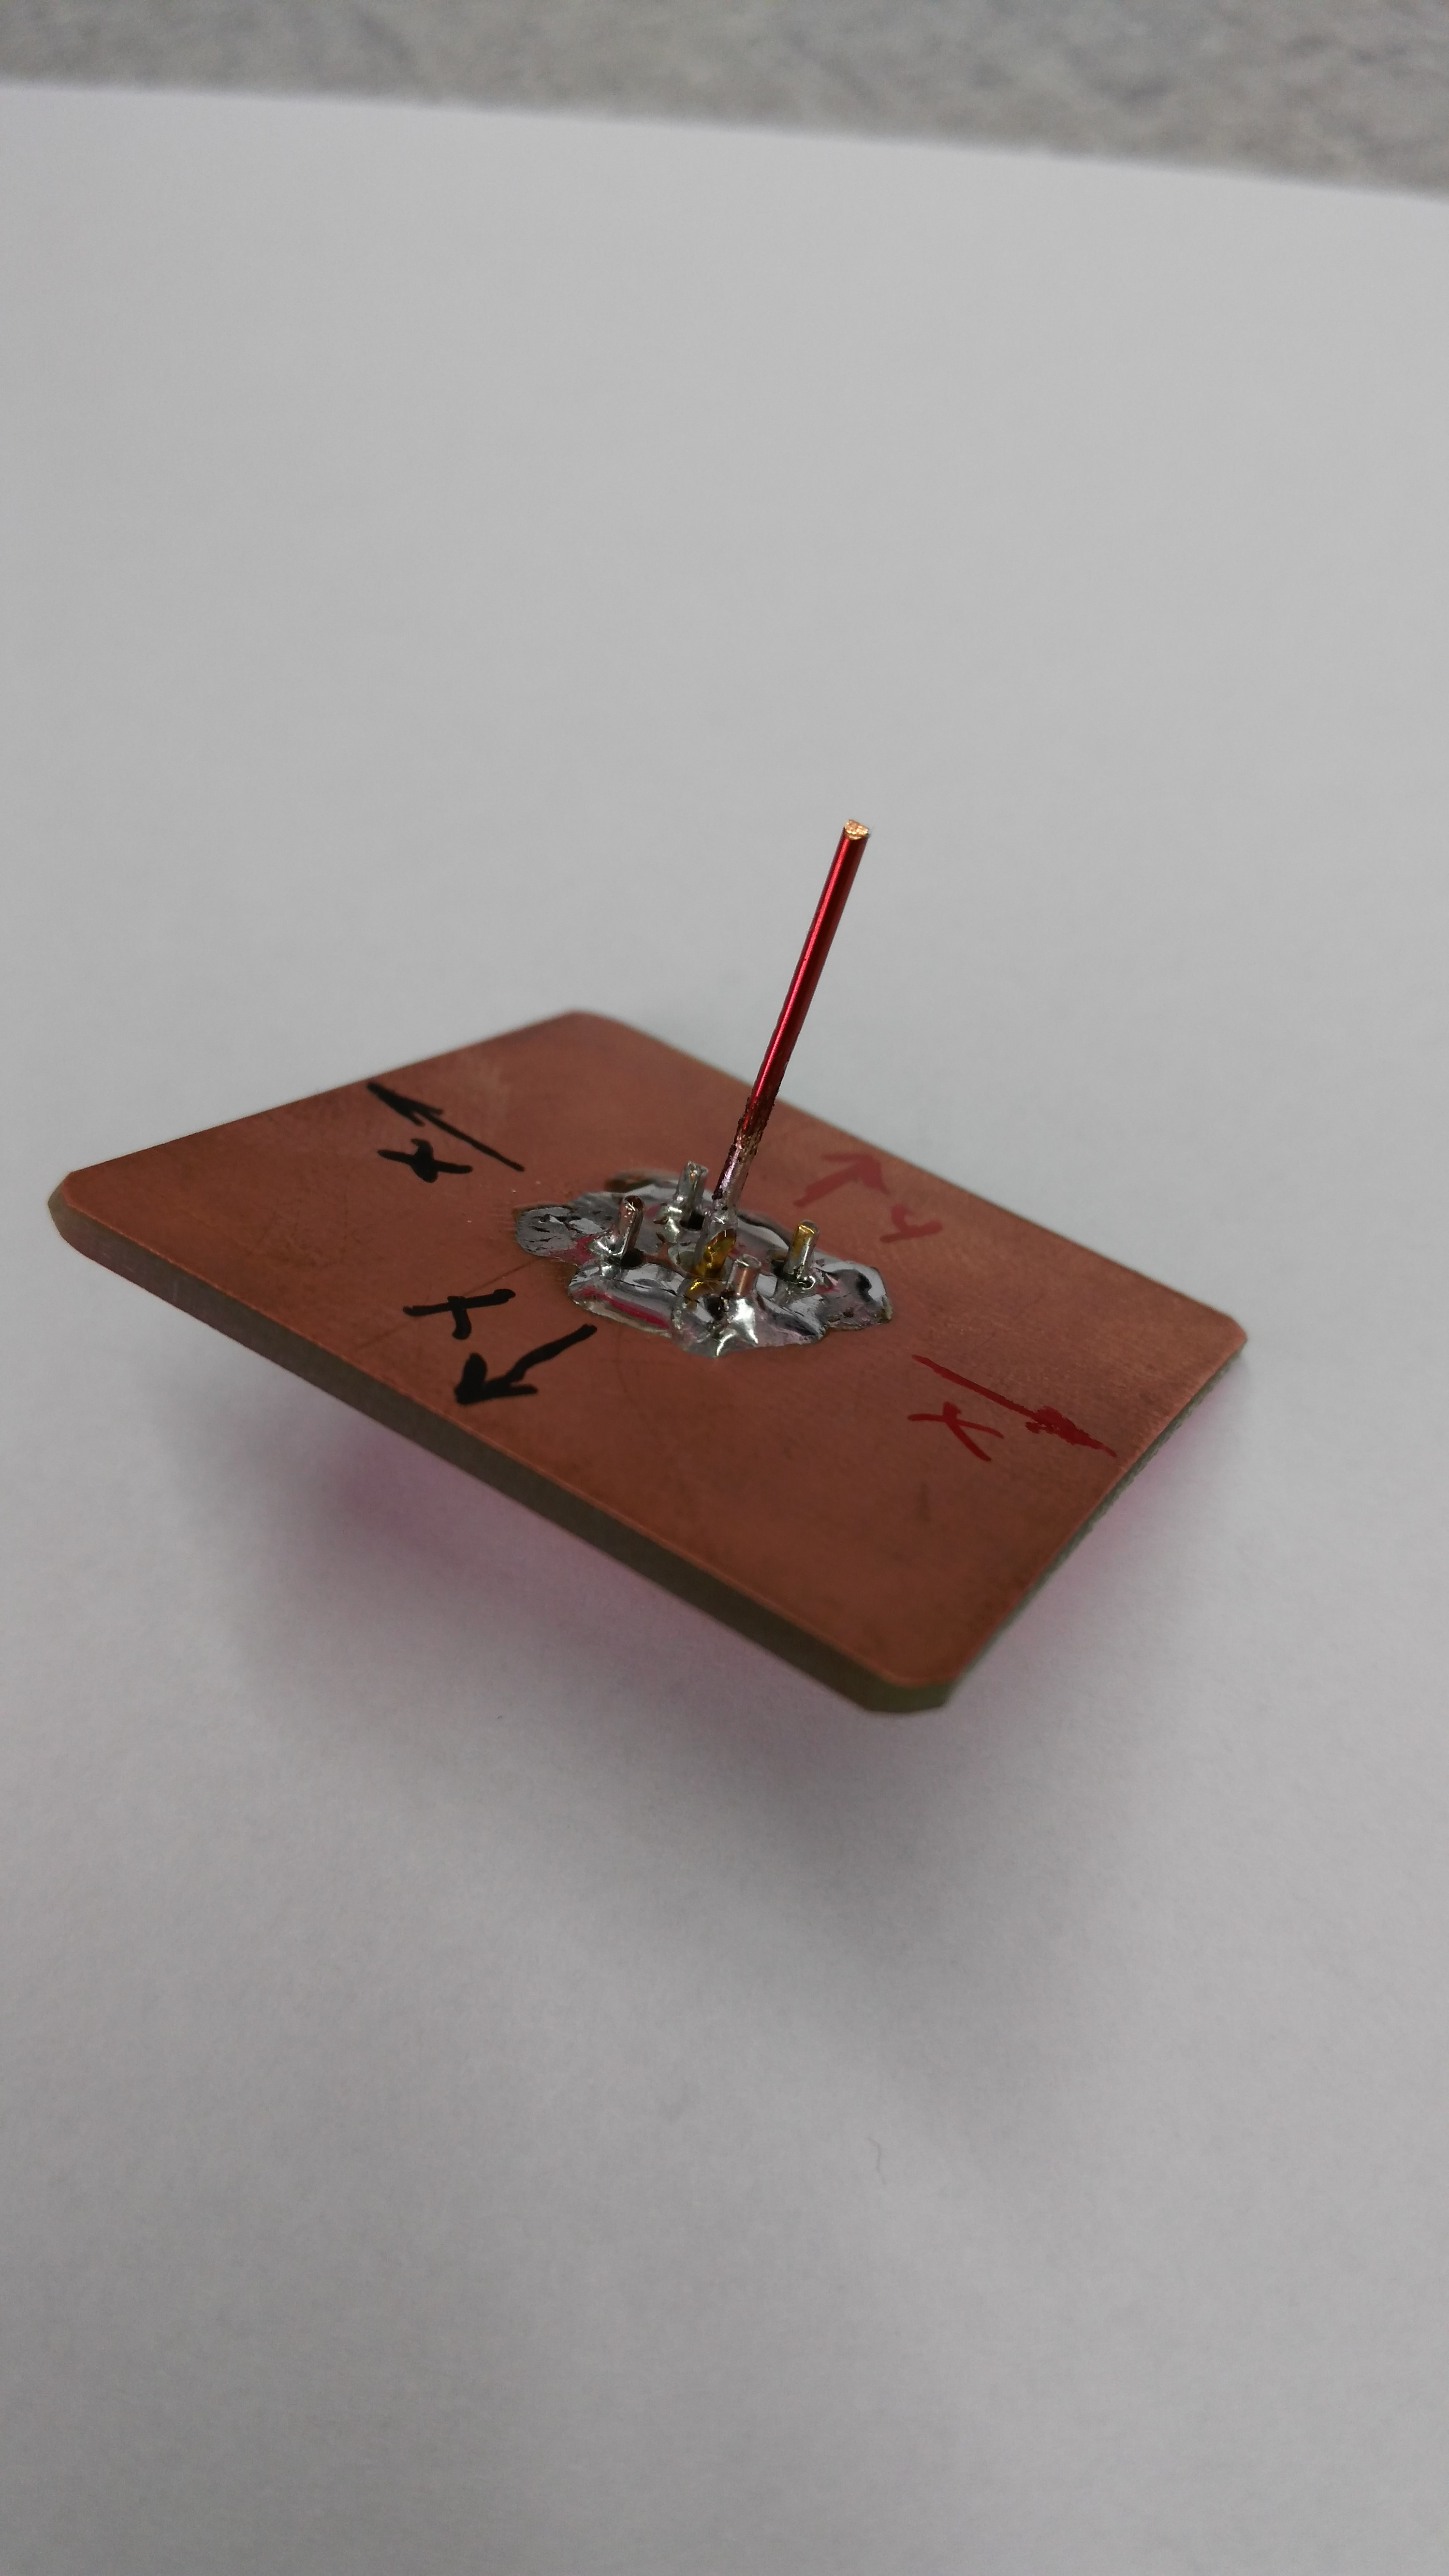
\includegraphics[width=0.22\textwidth]{../fig/pic/monopol_model_4.jpg}
%	\caption{Bilder der erstellten Monopolantenne.}
%\end{figure}



\clearpage
\subsubsection{Reflexion ($S_{11}$) und Impedanz}

\begin{figure}[h!]
	\centering
	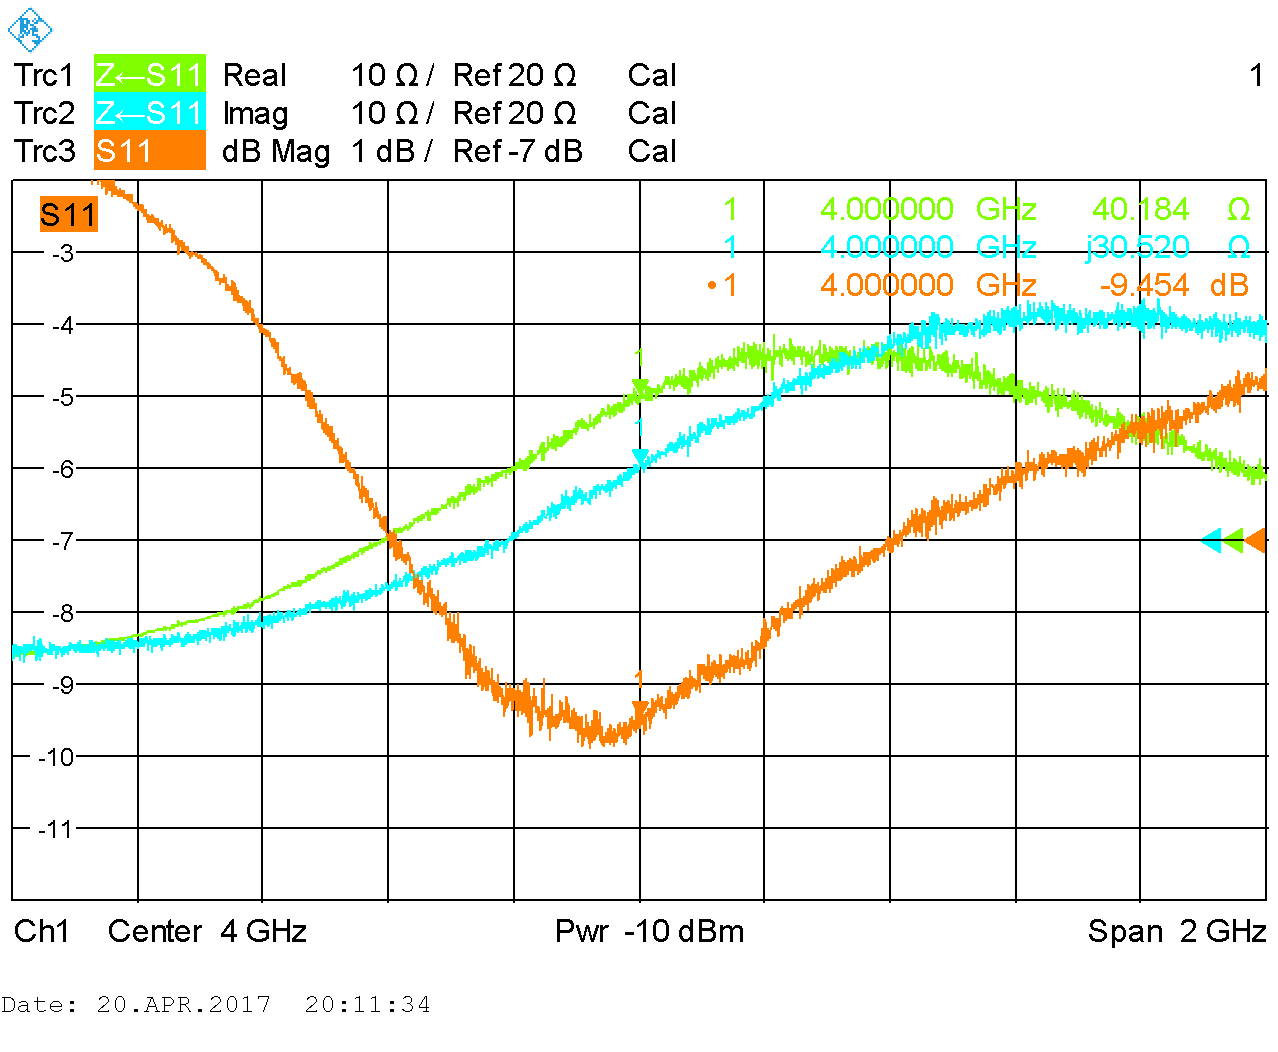
\includegraphics[width=0.75\textwidth]{../data/measurement/T2.png}
	\caption{Messung des Streuparameters $S_{11}$ (Reflexion) und der Impedanz $Z$}
\end{figure}

%\begin{figure}[h!]
%	\begin{subfigure}[t]{0.8\textwidth}
%		\centering
%		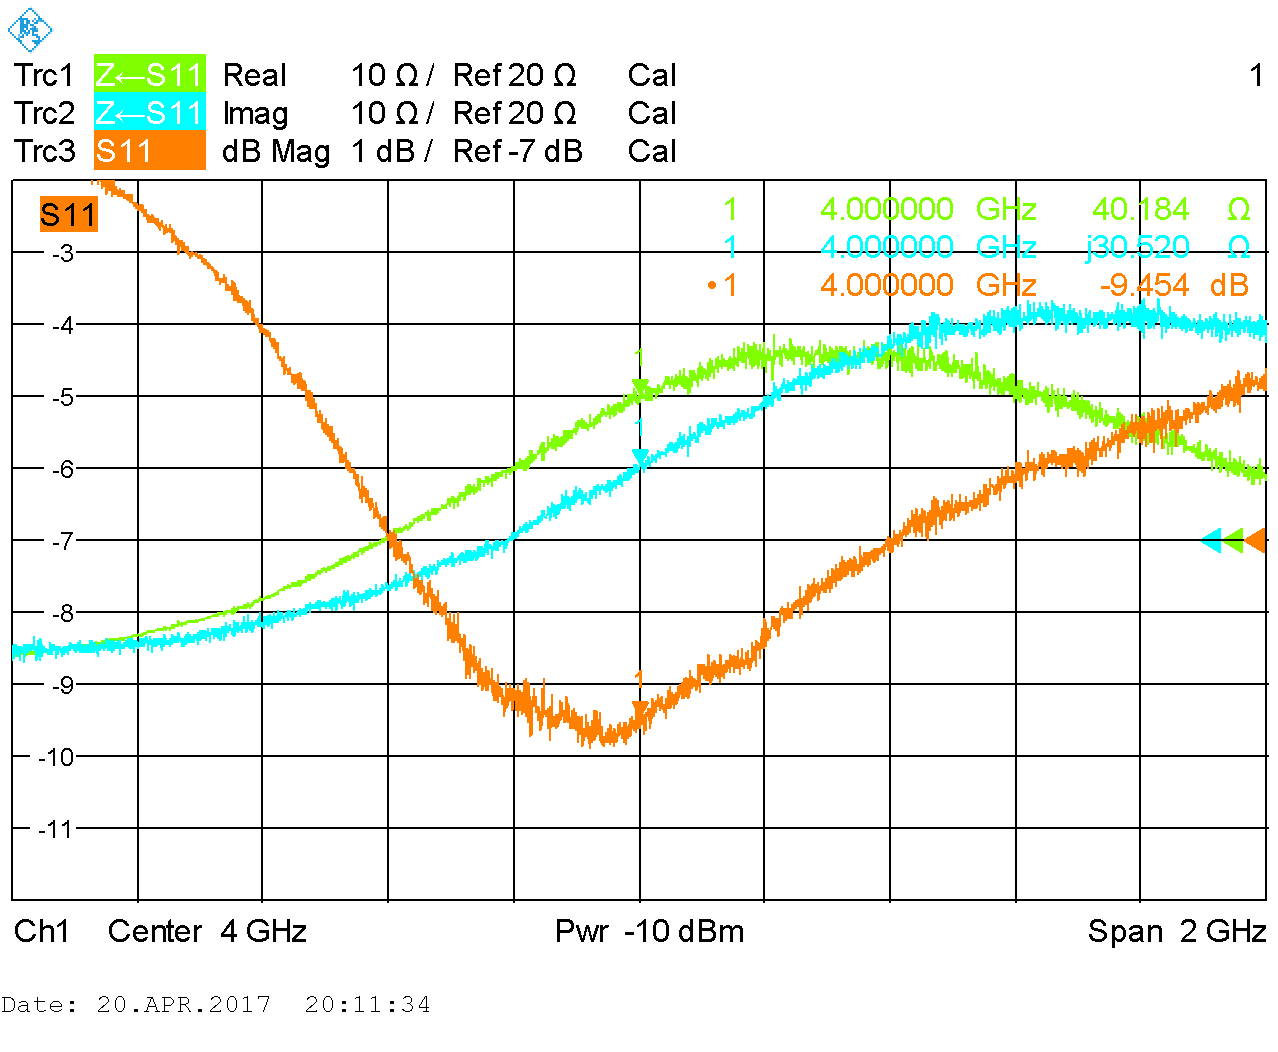
\includegraphics[width=1\textwidth]{../data/measurement/T2.png}
%		\caption{Messbild von $S_{11}$ und $Z$ mittels VNA }
%	\end{subfigure}
%
%	\begin{subfigure}[t]{0.8\textwidth}
%		\centering
%		\begin{tikzpicture}
%			\begin{axis}[
%				title=\textbf{Reflexion $S_{11}$ (VNA2)},
%				width=\textwidth,
%				height=0.5\textwidth,
%				grid=major,
%				grid style={dashed,gray!30},
%				xlabel={Frequenz [\si{\giga\hertz}]},
%				ylabel={$S_{11}$ [\si{\decibel}]},
%				x label style={at={(axis description cs:0.5,-0.075)},anchor=north},
%				legend style={at={(0.98,0.98)},anchor=north east},
%				x tick label style={rotate=90,anchor=east},
%				legend columns=1,
%				]
%				\addplot+[mark=none] table[x=f, y=s11, col sep=comma]{../data/measurement/vna_2_data.txt};
%				%\addlegendentry{S11};
%			\end{axis}
%		\end{tikzpicture}
%		\caption{V}
%	\end{subfigure}
%	\caption{Messung am Einspeisepunkt mit Vector-Network Analyser.}
%\end{figure}

Die Messungen mit dem Vector-Network Analyser zeigen, dass die erzielte
Frequenz ca. \SI{4}{\giga\hertz} beträgt (mit leichter Abweichung nach
unten). Die gemessene Impedanz liegt bei
$\mathrm{Re}\left\{Z\right\} \approx \SI{40}{\ohm}$ und
$\mathrm{Im}\left\{Z\right\} \approx \SI{31}{\ohm}$, was nahe den
simulierten Werten von \SI{50}{\ohm} respektive \SI{30}{\ohm} liegt.
Weiter ist auch der simulierte Resonanzpunkt nahe oberhalb der
\SI{4}{\giga\hertz} zu erkenen (im Bereich von \SI{4.4}{\giga\hertz}
$\dots$ \SI{4.8}{\giga\hertz}).


\clearpage
\subsubsection{Abstrahlung}

\begin{figure}[h!]
	\centering
	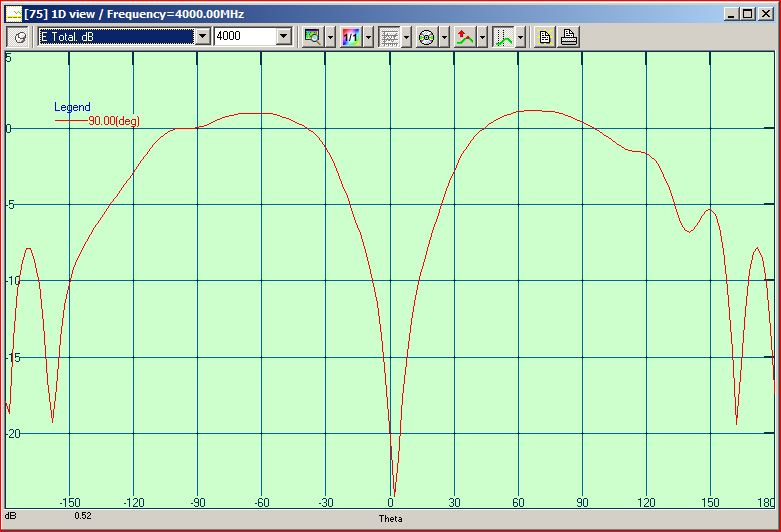
\includegraphics[width=0.75\textwidth]{../data/measurement/measurement_star_90deg_cut.JPG}
	\caption{Messung der Abstrahlung.}
\end{figure}

%\begin{figure}[h!]
%	\begin{subfigure}[t]{0.8\textwidth}
%		\centering
%		\begin{tikzpicture}
%			\begin{axis}[
%				title=\textbf{Abstrahlung},
%				width=\textwidth,
%				height=0.5\textwidth,
%				grid=major,
%				grid style={dashed,gray!30},
%				xlabel={Frequenz [\si{\giga\hertz}]},
%				ylabel={$S_{11}$ [\si{\decibel}]},
%				x label style={at={(axis description cs:0.5,-0.075)},anchor=north},
%				legend style={at={(0.98,0.98)},anchor=north east},
%				x tick label style={rotate=90,anchor=east},
%				legend columns=1,
%				each nth point=100
%				]	
%				\addplot+[mark=none] table[x index = {0}, y index = {1}, col sep=comma]{../data/measurement/data_etot.txt};
%				%\addlegendentry{S11};
%			\end{axis}
%		\end{tikzpicture}
%	\end{subfigure}
%	\caption{Messung der Abstrahlung.}
%\end{figure}

Die Messung der Abstrahlung (mit StarLab) zeigt wie bereits die Simulation,
dass in Richtung des Stabes (entlag der $z$-Achse, $\theta=\SI{0}{\degree}$) ein
Minimum vorliegt. Betrachtet man die Messergebnisse genauer, so ist ein
leichter \emph{tilt} (Schieflage) des Stabes zu erkennen, denn das
Minimum liegt nicht bei exakt $\theta=\SI{0}{\degree}$ sondern bei
$\theta > \SI{0}{\degree}$. Weiter ist zu erkennen, dass das Maximum
nicht wie erwartet bei $\theta=\SI{90}{\degree}$ (senkrecht zum Stab)
sondern bei ca. $\theta \pm \SI{60}{\degree}$ liegt. Als weitere
Abweichung zur Simulation ist zu erkennen, dass zum einen keine
Symmetrie vorliegt für $E_{\mathrm{total}}$ in den Punkten
bei $\theta \pm \SI{90}{\degree}$ und zum anderen auch ein
\emph{unruhiger} Verlauf zwischen
$\pm \SI{120}{\degree} \dots \pm \SI{180}{\degree}$ vorliegt.

%\subsubsection{Messaufbau}
%
%\subsubsection{Messmittel}
%
%
